\documentclass[11pt,a4paper]{article}

\usepackage[T1]{fontenc}
\usepackage[utf8]{inputenc}
\usepackage{amsmath,amssymb,amsthm}
\usepackage{booktabs,array,tabularx}
\usepackage{graphicx}
\usepackage{tikz}
\usetikzlibrary{arrows.meta,calc}
\usepackage[numbers,sort&compress]{natbib}
\usepackage{xcolor}
\usepackage{xurl}
\usepackage{microtype}
\usepackage{titling}
\usepackage{fancyhdr}
\usepackage{listings}
\usepackage[a4paper,margin=25mm]{geometry}
\usepackage[
  unicode=true,
  colorlinks=true,
  linkcolor=blue,
  citecolor=blue,
  urlcolor=blue
]{hyperref}

\graphicspath{{./}}
\urlstyle{same}

% Discreet horizontal rules in the running header and footer.
\setlength{\headheight}{14pt}
\pagestyle{fancy}
\fancyhf{}
\fancyfoot[C]{\thepage}
\renewcommand{\headrulewidth}{0.4pt}
\renewcommand{\footrulewidth}{0.4pt}
\fancypagestyle{plain}{%
  \fancyhf{}%
  \fancyfoot[C]{\thepage}%
  \renewcommand{\headrulewidth}{0.4pt}%
  \renewcommand{\footrulewidth}{0.4pt}%
}


% Python source code reproduced in the appendix.
\lstdefinestyle{paperpython}{
  language=Python,
  basicstyle=\ttfamily\scriptsize,
  columns=fullflexible,
  keepspaces=true,
  breaklines=true,
  breakatwhitespace=false,
  showstringspaces=false,
  numbers=left,
  numberstyle=\tiny\color{gray},
  numbersep=9pt,
  frame=single,
  framesep=4pt,
  xleftmargin=1.7em,
  framexleftmargin=1.5em,
  captionpos=t,
  aboveskip=1.2em,
  belowskip=1em
}

\newcommand{\be}{\begin{equation}}
\newcommand{\ee}{\end{equation}}
\newcommand{\lb}[1]{\label{#1}}
\newcommand{\e}{\mathrm{e}}
\newcommand{\dd}{\mathrm{d}}
\newcommand{\R}{\mathbb{R}}
\DeclareMathOperator{\tr}{tr}
\DeclareMathOperator{\Vol}{Vol}

\theoremstyle{definition}
\newtheorem{definition}{Definition}[section]
\newtheorem{theorem}{Theorem}[section]
\newtheorem{lemma}{Lemma}[section]
\newtheorem{proposition}{Proposition}[section]
\newtheorem{corollary}{Corollary}[section]
\newtheorem{example}{Example}[section]
\newtheorem{exercise}{Exercise}[section]
\newtheorem{remark}{Remark}[section]

\newenvironment{solution}
{\par\noindent\textbf{Solution.}}
{\hfill$\square$\par}

\numberwithin{equation}{section}

\title{From Abel's Identity to Liouville's Formula:\\
Determinants, Volume Evolution, and Applications in Dynamical Systems and Physics}

\author{Osvaldo L. Santos-Pereira\thanks{\href{mailto:olsp@if.ufrj.br}{olsp@if.ufrj.br}\quad\textbullet\quad
\href{https://orcid.org/0000-0003-2231-517X}{ORCID: 0000-0003-2231-517X}}\\
\small Physics Institute, Universidade Federal do Rio de Janeiro (UFRJ), Rio de Janeiro, Brazil}
\date{}
\setlength{\droptitle}{-2.2em}
\pretitle{\begin{center}\LARGE\bfseries}
\posttitle{\par\end{center}\vspace{-0.7em}}
\preauthor{\begin{center}\normalsize\begin{tabular}[t]{c}}
\postauthor{\end{tabular}\par\end{center}\vspace{-1.45em}}
\predate{}
\postdate{}
\renewenvironment{abstract}{%
  \small
  \begin{center}\bfseries Abstract\end{center}%
  \vspace{-0.55em}\noindent
}{\par\vspace{0.25em}}
\begin{document}
\maketitle

\begin{abstract}
Liouville's formula relates the determinant of a fundamental matrix of a linear ordinary differential system to the time integral of the trace of its coefficient matrix. This paper develops the formula from Abel's Wronskian identity, Jacobi's determinant formula, and the geometry of linear flows. Fundamental and state-transition matrices are introduced under explicit hypotheses, and the determinant is interpreted as a finite-time volume factor generated by the linear vector field. The framework yields higher-order Abel identities, spectral constraints for constant and periodic systems, and the Jacobian evolution of nonlinear flows. Applications to fluid mechanics, dissipative and parametrically driven oscillators, Hamiltonian dynamics, continuum mechanics, and Friedmann--Lema\^itre--Robertson--Walker (FLRW) cosmology show how the same determinant--trace relation controls volume evolution across several physical settings.
\end{abstract}
{\small\noindent\textbf{Keywords:} Abel identity; Liouville formula; Jacobi formula; fundamental matrix; state-transition matrix; determinant; trace; volume preservation; Floquet theory; dynamical systems.\par}
\vspace{0.35em}
\section*{Glossary of Terms and Symbols}
\addcontentsline{toc}{section}{Glossary of Terms and Symbols}
\begingroup
\footnotesize
\renewcommand{\arraystretch}{1.0}
\setlength{\tabcolsep}{2pt}
\noindent\begin{minipage}[t]{0.493\textwidth}
\vspace{0pt}
\begin{tabularx}{\linewidth}{@{}>{\raggedright\arraybackslash}p{0.30\linewidth}>{\raggedright\arraybackslash}X@{}}
\toprule
\textbf{Entry} & \textbf{Definition} \\
\midrule
$A(t)$ & Coefficient matrix of a linear system. \\
$M_n(\R)$ & Real $n\times n$ matrices. \\
$GL(n,\R)$ & Invertible real $n\times n$ matrices. \\
$I_n$ & Identity matrix of order $n$. \\
$U(t)$ & Fundamental matrix of $U'=AU$. \\
$\Phi(t,\tau)$ & State-transition matrix. \\
$\mathbf b(t)$ & External forcing in a linear system. \\
$\det B$ & Determinant; oriented volume factor. \\
$\tr B$ & Sum of the diagonal entries of $B$. \\
$W(t)$ & Wronskian of scalar solutions. \\
$\delta(t)$ & Determinant of normalized transport. \\
$\nabla\cdot\mathbf f$ & Divergence of a vector field. \\
$DF$ & Jacobian matrix of a differentiable map. \\
$\varphi_{t,t_0}$ & Nonlinear flow map from $t_0$ to $t$. \\
$X(t)$ & Variational matrix of the flow. \\
$R,S$ & Orthogonal and positive polar factors. \\
Abel & Wronskian evolution identity. \\
Jacobi & Differential identity for a determinant. \\
Liouville & Trace-controlled determinant evolution. \\
ODE & Ordinary differential equation. \\
\bottomrule
\end{tabularx}
\end{minipage}\hfill
\begin{minipage}[t]{0.493\textwidth}
\vspace{0pt}
\begin{tabularx}{\linewidth}{@{}>{\raggedright\arraybackslash}p{0.30\linewidth}>{\raggedright\arraybackslash}X@{}}
\toprule
\textbf{Entry} & \textbf{Definition} \\
\midrule
$\Vol(\Omega)$ & Lebesgue volume of a region. \\
$F$ & Deformation gradient of a material map. \\
$\mathcal J$ & Material Jacobian $\det F$. \\
$L$ & Spatial velocity-gradient matrix. \\
$J$ & Canonical symplectic matrix. \\
$\mathcal H$ & Hamiltonian function. \\
$K$ & Symmetric quadratic Hamiltonian matrix. \\
$\Theta$ & Expansion scalar of a congruence. \\
$\sigma_i$ & Singular values of the transition matrix. \\
$\ell_i$ & Asymptotic singular-value growth rates. \\
$\mu_j$ & Floquet multipliers of the monodromy. \\
$\nu_j$ & Floquet exponents: $\mu_j=\exp(T\nu_j)$. \\
$M$ & Monodromy matrix of a periodic system. \\
$H(t)$ & Hubble parameter $a'/a$. \\
$\boldsymbol\chi$ & Motion map of continuum mechanics. \\
$a(t)$ & Cosmological scale factor. \\
$k$ & FLRW spatial-curvature parameter. \\
$h_{ij}$ & Induced spatial metric in FLRW. \\
$V_{\rm phys}$ & Physical volume of a comoving region. \\
FLRW & Friedmann--Lema\^itre--Robertson--Walker. \\
\bottomrule
\end{tabularx}
\end{minipage}
\endgroup
\clearpage
\begingroup
\footnotesize
\setlength{\parskip}{0pt}
\tableofcontents
\endgroup
\clearpage
\section{Introduction}

Linear ordinary differential systems provide a setting in which algebraic, analytic, and geometric information can be separated and then recombined. A continuous matrix-valued coefficient determines an instantaneous linear generator; a fundamental matrix propagates complete initial data; its determinant records oriented volume change; and the trace of the generator controls the logarithmic rate of that change. Liouville's formula expresses this relation and links the classical Wronskian theory of Abel to matrix analysis and dynamical systems \cite{coddington1955,hartman2002,teschl2012,horn2013}.

The scalar Wronskian relation is conventionally called Abel's identity, while the higher-order determinant evolution and the determinant differentiation formula are associated with Liouville and Jacobi. The relevant nineteenth-century bibliographic sources are cited alongside the modern reference for Abel's identity \cite{abel1827,liouville1838,jacobi1841,dlmf_abel}. The present paper develops these results in their modern matrix form from first principles. The scalar starting point is Abel's identity for a second-order homogeneous equation. The scalar equation is converted constructively into first-order matrix form, after which the Wronskian becomes the determinant of a matrix solution. The algebraic ingredients required later are then isolated: determinant multiplicativity, the first variation of the determinant, cyclic invariance of the trace, and the Jacobian interpretation of determinant magnitude. This separation allows Jacobi's determinant formula and Liouville's formula to be stated under explicit hypotheses and proved without suppressing intermediate steps.

A second objective is geometric. A normalized fundamental matrix acts on the initial state space as a time-dependent linear deformation. Its columns describe the evolution of basis directions, the associated transition matrix transports arbitrary initial data, and its determinant measures the volume multiplication factor of transported regions. The trace enters because it is the divergence of the corresponding linear vector field. This geometric viewpoint provides the organizing interpretation that connects the algebraic theorem with the physical applications developed later.

The paper also develops consequences that are often presented separately. These include the higher-order Abel identity, the relation between trace and mean logarithmic volume growth, the product of Floquet multipliers for periodic systems, and the extension to the differential of a nonlinear flow through the variational equation. Applications are then given in fluid mechanics, damped and parametrically driven oscillators, Hamiltonian dynamics, continuum mechanics, and relativistic cosmology. The aim is to show that the determinant--trace relation is a structural statement that recurs whenever local linearization governs the evolution of volume.

\section{Abel's Identity}

Abel's identity is the scalar precursor of Liouville's formula and provides a direct route to the matrix theorem. For a second-order homogeneous linear equation, the identity determines the Wronskian of two solutions without requiring closed-form expressions for those solutions. The structural point is that a determinant-like quantity satisfies a closed first-order equation whose coefficient is read from the original differential equation. In the matrix generalization, the scalar Wronskian becomes the determinant of a fundamental matrix and the coefficient of the first derivative becomes the matrix trace \cite{coddington1955,hartman2002,teschl2012}.

\subsection{Wronskian of a Second-Order Equation}

As the scalar prototype, consider a second-order homogeneous linear equation written in standard form so that the coefficient of the highest derivative is unity:
\be
y''+p(t)y'+q(t)y=0,
\lb{eq:abel-ode}
\ee
where $p,q:I\rightarrow\R$ are continuous on an interval $I$. Continuity is sufficient for the usual existence and uniqueness theory for the corresponding initial-value problem, and any solution is determined by the two initial data $y(t_0)$ and $y'(t_0)$ \cite{coddington1955,teschl2012}. Let $y_1$ and $y_2$ be two solutions. Their Wronskian is defined by
\be
W(t)=
\det
\begin{pmatrix}
y_1(t) & y_2(t)\\
y_1'(t) & y_2'(t)
\end{pmatrix}
=
y_1y_2'-y_2y_1'.
\lb{eq:abel-wronskian}
\ee
The determinant carries the linear-independence information of the two state vectors. The two columns are the state vectors $(y_1,y_1')^{\mathsf T}$ and $(y_2,y_2')^{\mathsf T}$ of the associated first-order system, so $W(t_0)\neq0$ is the condition that these two states are linearly independent at $t_0$. Because the solution space of a second-order homogeneous linear equation is two-dimensional, a pair with nonzero Wronskian forms a basis of that solution space. Abel's identity will show that the Wronskian cannot vanish at any later time if it is nonzero initially; its nonvanishing is propagated by the differential equation itself.

\subsection{Abel's Formula and Direct Derivation}

The Wronskian satisfies an equation that contains $p(t)$ but not $q(t)$. Although both coefficients enter the differential equation, the $q(t)$ contribution cancels after differentiating the determinant. Writing that cancellation step by step prepares the row-by-row proof of Liouville's formula used later.

\begin{theorem}[Abel's identity]
For the equation in Eq.~\eqref{eq:abel-ode}, the Wronskian of any two solutions satisfies
\be
W(t)=W(t_0)
\exp\left[-\int_{t_0}^{t}p(s)\,\dd s\right].
\lb{eq:abel-identity}
\ee
\end{theorem}

\begin{exercise}[Derivation of Abel's identity]
Starting from the definition in Eq.~\eqref{eq:abel-wronskian}, derive Eq.~\eqref{eq:abel-identity} from the differential equation.
\end{exercise}

\begin{solution}
Differentiate the Wronskian with respect to time. The product rule gives four terms,
\be
W'
=
y_1'y_2'+y_1y_2''-y_2'y_1'-y_2y_1''.
\lb{eq:abel-step1}
\ee
The first and third terms cancel because scalar multiplication is commutative. Therefore
\be
W'=y_1y_2''-y_2y_1''.
\lb{eq:abel-step2}
\ee
Each solution satisfies Eq.~\eqref{eq:abel-ode}; solving that equation for the second derivative gives
\be
y_i''=-p(t)y_i'-q(t)y_i,
\qquad i=1,2.
\lb{eq:abel-second}
\ee
Substituting these two expressions into Eq.~\eqref{eq:abel-step2} yields
\be
W'
=
y_1(-py_2'-qy_2)-y_2(-py_1'-qy_1).
\lb{eq:abel-step3}
\ee
The terms proportional to $q(t)$ cancel because $-qy_1y_2+qy_2y_1=0$. The remaining terms factor as
\be
W'=-p(t)\bigl(y_1y_2'-y_2y_1'\bigr).
\lb{eq:abel-step4}
\ee
The expression in parentheses is $W(t)$, so the second-order problem has reduced to the scalar first-order equation
\be
W'=-p(t)W.
\lb{eq:abel-scalar}
\ee
To solve this first-order equation without assuming in advance that $W$ is nonzero, introduce the integrating factor
\begin{equation}
\mu(t)=\exp\left[\int_{t_0}^{t}p(s)\,\dd s\right].
\end{equation}
Its derivative is $\mu'(t)=p(t)\mu(t)$. Multiplying Eq.~\eqref{eq:abel-scalar} by $\mu(t)$ gives
\begin{equation}
\mu W'+p\mu W=0,
\end{equation}
and the left-hand side is exactly the derivative of the product $\mu W$. Indeed, using $\mu'=p\mu$ in the product rule gives
\begin{equation}
\frac{\dd}{\dd t}\bigl[\mu(t)W(t)\bigr]=0.
\end{equation}
The product is therefore constant on $I$, so $\mu(t)W(t)=\mu(t_0)W(t_0)=W(t_0)$. Solving for $W(t)$ gives Eq.~\eqref{eq:abel-identity}. Because the exponential factor never vanishes, the formula also proves that $W$ is either identically zero or never zero on a connected interval. Thus linear independence, once present at one time, persists throughout the interval \cite{coddington1955,hartman2002,teschl2012}.
\end{solution}

The disappearance of $q(t)$ has a precise determinant interpretation. The coefficient $q$ acts in the component of the first-order system that mixes position into velocity, but it does not contribute to the trace of the companion matrix. The coefficient $p(t)$, by contrast, appears on the diagonal and therefore controls the net infinitesimal area rate in the two-dimensional state space. This observation already contains the main conceptual transition from Abel to Liouville.

\subsection{First-Order Matrix Form and Liouville Preview}

The passage from the scalar equation to a first-order system can be constructed component by component. Define two state variables by
\begin{equation}
x_1(t)=y(t),
\qquad
x_2(t)=y'(t),
\end{equation}
and collect them into the column vector $\mathbf{x}=(x_1,x_2)^{\mathsf T}=(y,y')^{\mathsf T}$. Differentiating the first definition gives $x_1'=x_2$. The original equation, Eq.~\eqref{eq:abel-ode}, determines the derivative of the second state variable because $x_2'=y''$. Solving the scalar equation for $y''$ and replacing $y$ and $y'$ by $x_1$ and $x_2$ gives
\begin{equation}
x_2'=-q(t)x_1-p(t)x_2.
\end{equation}
The two scalar first-order equations are therefore
\begin{equation}
x_1'=0\,x_1+1\,x_2,
\qquad
x_2'=-q(t)x_1-p(t)x_2.
\end{equation}
Reading the coefficients of $x_1$ and $x_2$ row by row produces the companion matrix and yields
\be
\mathbf{x}'
=
\begin{pmatrix}
0 & 1\\
-q(t) & -p(t)
\end{pmatrix}
\mathbf{x}.
\lb{eq:abel-system}
\ee
Thus Eq.~\eqref{eq:abel-system} is not an additional assumption: its first row encodes the definition $x_2=y'$, while its second row is the original second-order equation solved for $y''$. This rewriting changes the problem from a scalar second-order equation to a first-order matrix system. It converts the scalar equation into the general first-order form $\mathbf{x}'=A(t)\mathbf{x}$, allowing the Wronskian to be recognized as an ordinary matrix determinant. If the two columns of a matrix $U(t)$ are the state vectors $(y_1,y_1')^{\mathsf T}$ and $(y_2,y_2')^{\mathsf T}$, then $U'=AU$ and
\be
\det U(t)=W(t).
\lb{eq:abel-det-U}
\ee
The companion matrix has only one coefficient from the scalar differential equation on its diagonal. Summing those diagonal entries, which by definition gives the trace of a square matrix, yields
\be
\tr A(t)=-p(t),
\lb{eq:abel-trace}
\ee
because its diagonal entries are $0$ and $-p(t)$. Abel's identity can therefore be rewritten as
\be
W(t)=W(t_0)
\exp\left[
\int_{t_0}^{t}\tr A(s)\,\dd s
\right].
\lb{eq:abel-matrix-preview}
\ee
This form contains no feature specific to dimension two except the size of the determinant. Liouville's formula states that the same relation holds for the determinant of a fundamental matrix of an arbitrary $n$-dimensional first-order linear system. The later proof will therefore generalize two elements that are already visible here: the Wronskian becomes $\det U$, and the scalar coefficient $-p(t)$ becomes $\tr A(t)$.

%%%%%%%%%%%%%%%%%%%%%%%%%%%%%%%%%%%%%%%%%%%%%%%%%%%%%%%%%%%%%%%%%%%%%%%
\section{Algebraic Preliminaries}

This section collects the algebraic and analytic facts used in the proof of Liouville's formula. The determinant converts matrix composition into volume multiplication, its first variation produces the trace, cyclicity makes the trace invariant under similarity, and Jacobian determinants connect these algebraic operations with changes of variables. The final ingredient is the scalar first-order equation that governs the determinant of a fundamental matrix. The purpose of separating these results is to make every later step refer to a specific property rather than treating determinant and trace identities as formal manipulations \cite{horn2013,coddington1955,hartman2002,teschl2012}.

\subsection{Matrix Notation and Existence Assumptions}

Let $I\subset\R$ be an interval and let $A:I\rightarrow M_n(\R)$ be continuous. The general homogeneous system considered throughout the paper is
\be
\frac{\dd\mathbf{x}}{\dd t}=A(t)\mathbf{x},
\qquad
\mathbf{x}(t)\in\R^n.
\lb{eq:system}
\ee
Vectors are written in boldface and are understood as columns. The symbol $M_n(\R)$ denotes the vector space of real $n\times n$ matrices, $GL(n,\R)$ denotes the group of invertible matrices in $M_n(\R)$, and $I_n$ denotes the identity matrix. For a square matrix $B$, the trace is
\be
\tr B=\sum_{i=1}^{n}B_{ii}.
\lb{eq:trace-definition}
\ee
The notation $\Vol(\Omega)$ denotes the $n$-dimensional Lebesgue volume of a measurable region $\Omega\subset\R^n$. A prime denotes differentiation with respect to $t$.

Continuity of $A$ is sufficient for the standard existence and uniqueness theorem for linear systems. Thus, for each $t_0\in I$ and each $\mathbf{x}_0\in\R^n$, there exists a unique solution of Eq.~\eqref{eq:system} satisfying $\mathbf{x}(t_0)=\mathbf{x}_0$ \cite{coddington1955,hartman2002,teschl2012}. This fact makes the solution operator from one time to another a well-defined linear map on the full state space. In particular, the $n$ solutions generated by the canonical basis at $t_0$ assemble into a unique normalized fundamental matrix.

\subsection{Determinant Multiplicativity and First-Order Variation}

The determinant converts composition of linear maps into multiplication of scalar volume factors. For $B,C\in M_n(\R)$,
\be
\det(BC)=\det(B)\det(C).
\lb{eq:det-product}
\ee
Invertibility is equivalent to a nonzero determinant. Applying multiplicativity to $BB^{-1}=I_n$ then determines the determinant of the inverse:
\be
\det(B^{-1})=\frac{1}{\det B}.
\lb{eq:det-inverse}
\ee
These identities allow a differentiable matrix curve to be factored into its present value and a perturbation of the identity. The local behavior of that perturbation is encoded in the following lemma \cite{horn2013}.

\begin{lemma}[First variation of the determinant]
For $C\in M_n(\R)$ and $h\rightarrow0$,
\be
\det(I_n+hC)=1+h\tr C+O(h^2).
\lb{eq:det-linearization}
\ee
\end{lemma}

\begin{proof}
Write the columns of $C$ as $\mathbf c_1,\ldots,\mathbf c_n$. The $j$th column of $I_n+hC$ is $\mathbf e_j+h\mathbf c_j$. Multilinearity expands the determinant into terms obtained by choosing either $\mathbf e_j$ or $h\mathbf c_j$ from each column. The zeroth-order term is
\be
\det(\mathbf e_1,\ldots,\mathbf e_n)=1.
\lb{eq:det-firstvariation-zero}
\ee
The first-order contribution arises by selecting $h\mathbf c_j$ from exactly one column and the corresponding basis vector from every other column. Summing these $n$ contributions gives
\be
h\sum_{j=1}^{n}
\det(\mathbf e_1,\ldots,\mathbf c_j,\ldots,\mathbf e_n)
=
h\sum_{j=1}^{n}C_{jj}
=
h\tr C.
\lb{eq:det-firstvariation-linear}
\ee
To justify the coefficient $C_{jj}$, expand the determinant with column $\mathbf c_j$ along that column: the cofactors of all rows except $j$ vanish because the remaining columns are canonical basis vectors, and the $j$th cofactor is one. Every remaining term contains at least two factors of $h$ and is $O(h^2)$. Combining the contributions gives Eq.~\eqref{eq:det-linearization}. The proof also explains why the trace appears: it is the coefficient of the linear response of the determinant at the identity.
\end{proof}

\subsection{Trace Cyclicity and Similarity Invariance}

The trace is linear, but the property needed for Liouville's formula is its invariance under cyclic permutations of a product. For compatible square matrices $B$ and $C$, the diagonal of $BC$ gives
\be
\tr(BC)
=
\sum_{i=1}^{n}(BC)_{ii}
=
\sum_{i=1}^{n}\sum_{j=1}^{n}B_{ij}C_{ji}.
\lb{eq:trace-product-components}
\ee
Interchanging the dummy indices and using commutativity of scalar multiplication yields
\be
\sum_{i,j}B_{ij}C_{ji}
=
\sum_{j,i}C_{ji}B_{ij}
=
\tr(CB).
\lb{eq:trace-cyclic}
\ee
Thus $\tr(BC)=\tr(CB)$. This does not imply $BC=CB$; the cyclic property belongs to the trace, not to matrix multiplication.

A concrete $2\times2$ example makes the distinction explicit. Let
\be
B=
\begin{pmatrix}
1&2\\
0&3
\end{pmatrix},
\qquad
C=
\begin{pmatrix}
4&-1\\
2&1
\end{pmatrix}.
\lb{eq:trace-example-matrices}
\ee
To verify explicitly that cyclicity does not require commutativity, multiply the matrices in both orders. Direct matrix multiplication gives
\be
BC=
\begin{pmatrix}
8&1\\
6&3
\end{pmatrix},
\qquad
CB=
\begin{pmatrix}
4&5\\
2&7
\end{pmatrix}.
\lb{eq:trace-example-products}
\ee
The two products are plainly different, but their diagonal sums coincide. Evaluating those sums gives
\be
\tr(BC)=8+3=11=4+7=\tr(CB).
\lb{eq:trace-example-result}
\ee
Cyclicity also explains why the trace is independent of the matrix representation chosen for a linear operator. If $S\in GL(n,\R)$ changes basis, then the similar matrix $S^{-1}BS$ has trace
\be
\tr(S^{-1}BS)
=
\tr(BSS^{-1})
=
\tr B.
\lb{eq:trace-similarity}
\ee
This is the property that later reduces $\tr(U^{-1}AU)$ to $\tr A$. It also shows that the trace is an invariant of the linear operator, rather than of a chosen basis \cite{horn2013}.

\subsection{Jacobians and Volume Transformation}

Let $\Omega\subset\R^n$ be open and let $F:\Omega\rightarrow\R^n$ be continuously differentiable. Its Jacobian matrix at $\mathbf{x}\in\Omega$ is
\be
DF(\mathbf{x})=
\left(
\frac{\partial F_i}{\partial x_j}
\right)_{i,j=1}^{n}.
\lb{eq:jacobian}
\ee
If $F$ is injective and $\det DF(\mathbf x)\ne0$ throughout $\Omega$, the inverse-function theorem makes $F$ a continuously differentiable diffeomorphism onto its image. For the resulting change of variables $\mathbf y=F(\mathbf x)$,
\be
\dd^n y
=
|\det DF(\mathbf{x})|\,\dd^n x.
\lb{eq:volume-element}
\ee
The absolute value is required because geometric volume is nonnegative, whereas the sign of the determinant records orientation. For an invertible linear map $F(\mathbf x)=B\mathbf x$, the Jacobian matrix is the constant matrix $B$, and the measure-scaling identity $\Vol(B\Omega)=|\det B|\Vol(\Omega)$ holds for any Lebesgue-measurable region. This is the special case needed for linear flows \cite{apostol1969}.

The determinant of the Jacobian is most transparent when it is computed in familiar coordinate systems. The following examples show how the same determinant that later measures dynamical volume deformation already appears in elementary changes of variables.

\begin{example}[Polar coordinates]
On a regular polar chart with $r>0$ and an open angular interval of length $2\pi$ (excluding a cut ray), the polar map sends $(r,\theta)$ to $(x,y)$ according to
\be
x=r\cos\theta,
\qquad
y=r\sin\theta.
\lb{eq:polar-map}
\ee
Differentiating both Cartesian coordinates with respect to the new variables produces the Jacobian matrix. Its determinant measures the local area scaling of an infinitesimal rectangle in the $(r,\theta)$ plane:
\be
\frac{\partial(x,y)}{\partial(r,\theta)}
=
\begin{pmatrix}
\cos\theta & -r\sin\theta\\
\sin\theta & r\cos\theta
\end{pmatrix},
\qquad
\det\frac{\partial(x,y)}{\partial(r,\theta)}=r.
\lb{eq:polar-jacobian}
\ee
On the chosen regular polar chart $r>0$, so the Jacobian determinant is positive and its absolute value equals $r$. The Cartesian area element is therefore obtained by multiplying the coordinate area element by this local scale factor:
\be
\dd x\,\dd y=r\,\dd r\,\dd\theta.
\lb{eq:polar-area}
\ee
\end{example}

\begin{example}[Cylindrical coordinates]
Cylindrical coordinates extend a regular polar chart by leaving the axial coordinate unchanged. The axis and the angular cut are excluded from the diffeomorphic chart, although they have measure zero in volume integrals. With $x=\rho\cos\phi$, $y=\rho\sin\phi$, and the same coordinate $z$, differentiation gives
\be
\frac{\partial(x,y,z)}{\partial(\rho,\phi,z)}
=
\begin{pmatrix}
\cos\phi & -\rho\sin\phi & 0\\
\sin\phi & \rho\cos\phi & 0\\
0&0&1
\end{pmatrix},
\qquad
\det\frac{\partial(x,y,z)}{\partial(\rho,\phi,z)}=\rho.
\lb{eq:cylindrical-jacobian}
\ee
The third row and column contribute a unit factor, so the three-dimensional volume scaling is inherited directly from the planar polar transformation. Consequently, the cylindrical volume element is
\be
\dd V=\rho\,\dd\rho\,\dd\phi\,\dd z.
\lb{eq:cylindrical-volume}
\ee
\end{example}

\begin{example}[Spherical coordinates]
The spherical transformation introduces radial and angular dependence in all three Cartesian coordinates. Using $r>0$, $0<\theta<\pi$, and an open azimuthal interval of length $2\pi$, the coordinate map is
\be
x=r\sin\theta\cos\phi,
\qquad
y=r\sin\theta\sin\phi,
\qquad
z=r\cos\theta.
\lb{eq:spherical-map}
\ee
Differentiating the map with respect to $(r,\theta,\phi)$ produces three tangent vectors to the coordinate lines. Arranging these vectors as the columns of the Jacobian matrix gives
\be
\frac{\partial(x,y,z)}{\partial(r,\theta,\phi)}
=
\begin{pmatrix}
\sin\theta\cos\phi & r\cos\theta\cos\phi & -r\sin\theta\sin\phi\\
\sin\theta\sin\phi & r\cos\theta\sin\phi & r\sin\theta\cos\phi\\
\cos\theta & -r\sin\theta & 0
\end{pmatrix}.
\lb{eq:spherical-jacobian-matrix}
\ee
Expanding this determinant, or equivalently evaluating the scalar triple product of the three coordinate tangent vectors, yields the local volume scale factor
\be
\det\frac{\partial(x,y,z)}{\partial(r,\theta,\phi)}
=r^2\sin\theta.
\lb{eq:spherical-jacobian}
\ee
On the regular spherical chart specified above, $r>0$ and $0<\theta<\pi$, so this determinant is strictly positive. The corresponding Euclidean volume element therefore becomes
\be
\dd V=r^2\sin\theta\,\dd r\,\dd\theta\,\dd\phi.
\lb{eq:spherical-volume}
\ee
\end{example}

These three calculations show that the familiar factors $r$, $\rho$, and $r^2\sin\theta$ are not ad hoc corrections attached to particular coordinate systems; they are determinants of the corresponding Jacobian matrices. The same change-of-variables mechanism later identifies $\det\Phi(t,t_0)$ as the local and, for a linear flow, global volume factor generated by time evolution.

\subsection{Scalar Exponential Evolution}

The determinant equation produced by Jacobi's formula is scalar. Its integration is already illustrated by the proof of Abel's identity in Sec.~2.2, where an integrating factor is used without first assuming that the unknown function is nonzero. The same argument applies to the general homogeneous equation
\be
w'(t)=a(t)w(t),
\lb{eq:scalar-ode}
\ee
where $a:I\to\R$ is continuous. Multiplication by the integrating factor $\exp[-\int_{t_0}^{t}a(s)\,\dd s]$ makes the derivative of the corresponding product vanish, just as in the Wronskian calculation. Evaluation at the reference time therefore gives
\be
w(t)=w(t_0)
\exp\left[
\int_{t_0}^{t}a(s)\,\dd s
\right].
\lb{eq:scalar-solution}
\ee
The exponential factor is positive, so a solution that is nonzero at one time cannot cross zero. Liouville's formula will use this same scalar result with $w=\det U$ and $a=\tr A$ \cite{coddington1955,teschl2012}.


\section{Fundamental Matrix}

The fundamental matrix is the object that converts the scalar existence theory of a linear system into a linear transformation of the entire state space. Because the literature uses the term in several equivalent ways, we distinguish a general fundamental matrix from the normalized principal fundamental matrix, also called the state-transition matrix. The definitions and properties used below follow ODE references \cite{coddington1955,hartman2002,teschl2012}.

\subsection{The General Linear Group}

Before introducing fundamental matrices, it is useful to identify the natural algebraic space in which they take values. The coefficient matrix $A(t)$ may be any element of $M_n(\R)$, but a fundamental matrix must remain invertible at every time. The relevant set is therefore the \emph{general linear group}, denoted by $GL(n,\R)$, which consists of all invertible real $n\times n$ matrices:
\begin{equation}
GL(n,\R)
=
\left\{B\in M_n(\R):\det B\neq0\right\}.
\label{eq:GL-definition}
\end{equation}
The word ``group'' refers to matrix multiplication. If $B,C\in GL(n,\R)$, determinant multiplicativity shows that their product is again invertible because
\begin{equation}
\det(BC)=\det B\,\det C\neq0.
\label{eq:GL-closure}
\end{equation}
The identity matrix $I_n$ belongs to $GL(n,\R)$, every $B\in GL(n,\R)$ has an inverse $B^{-1}\in GL(n,\R)$, and associativity is inherited from ordinary matrix multiplication. These facts may be summarized by
\begin{equation}
BI_n=I_nB=B,
\qquad
BB^{-1}=B^{-1}B=I_n,
\qquad
\det(B^{-1})=\frac{1}{\det B}.
\label{eq:GL-identity-inverse}
\end{equation}
$GL(n,\R)$ is noncommutative for every $n\geq2$: two invertible matrices need not satisfy $BC=CB$. This distinction is important later, because identities such as $\tr(BC)=\tr(CB)$ rely on cyclicity of the trace rather than commutativity of matrix multiplication.

The determinant also separates $GL(n,\R)$ into orientation-preserving and orientation-reversing parts. Define
\begin{equation}
GL^{+}(n,\R)=\{B\in GL(n,\R):\det B>0\},
\qquad
GL^{-}(n,\R)=\{B\in GL(n,\R):\det B<0\}.
\label{eq:GL-components}
\end{equation}
A continuous curve in $GL(n,\R)$ cannot move from one of these sets to the other without passing through a matrix with zero determinant. Consequently, once a fundamental matrix is shown to be a continuous curve in $GL(n,\R)$, the sign of its determinant is fixed throughout the interval of existence. Liouville's formula will later sharpen this qualitative fact by giving the determinant explicitly as a function of time.

For constant generators, the matrix exponential provides a constructive curve in the general linear group. For $B\in M_n(\R)$ and real $t$, its convergent power series is
\be
\exp(tB)=\sum_{k=0}^{\infty}\frac{t^kB^k}{k!},\qquad B^0=I_n.
\lb{eq:matrix-exp-series}
\ee
The series converges absolutely in every submultiplicative matrix norm, since its terms are bounded by $|t|^k\|B\|^k/k!$, and uniformly on bounded time intervals. Termwise differentiation gives
\be
\frac{\dd}{\dd t}\exp(tB)=B\exp(tB),\qquad \exp(0B)=I_n.
\lb{eq:matrix-exp-derivative}
\ee
Because $tB$ and $-tB$ commute, the Cauchy product theorem for absolutely convergent matrix series applies to their exponential series. Combining equal powers gives $\exp(tB)\exp(-tB)=I_n$, so $\exp(tB)\in GL(n,\R)$. The existence-and-uniqueness theorem for linear initial-value problems, stated in Sec.~3.1, identifies $\exp[(t-t_0)B]$ as the unique normalized matrix solution of $\mathbf x'=B\mathbf x$. This construction will be used for constant generators.

\subsection{Matrix Solution}

The passage from individual vector solutions to a fundamental matrix consists of collecting a basis of solutions into a single matrix-valued curve. Let $\boldsymbol{\phi}_1,\ldots,\boldsymbol{\phi}_n$ be solutions of Eq.~\eqref{eq:system}. Assemble them as columns,
\be
U(t)=
\bigl[
\boldsymbol{\phi}_1(t)\ 
\boldsymbol{\phi}_2(t)\ 
\cdots\ 
\boldsymbol{\phi}_n(t)
\bigr].
\lb{eq:column-matrix}
\ee
Differentiation acts column by column. Since each column satisfies the same system,
\be
U'(t)=A(t)U(t).
\lb{eq:matrix-solution}
\ee
The matrix $U$ is called a \emph{fundamental matrix} when its columns are linearly independent. For $n$ vectors in $\R^n$, linear independence is equivalent to invertibility of the column matrix. Hence $U(t)$ is fundamental precisely when it lies in $GL(n,\R)$, or equivalently when
\be
\det U(t)\neq0.
\lb{eq:fundamental-det}
\ee
The determinant of a fundamental matrix is the matrix analogue of the Wronskian.

Initial invertibility of a matrix solution is sufficient to guarantee that it remains a fundamental matrix. This must be established without assuming the determinant formula under investigation.

\begin{proposition}[Persistence of invertibility]\label{prop:invertible}
Let $A:I\to M_n(\R)$ be continuous and let $X:I\to M_n(\R)$ satisfy $X'=AX$. If $X(t_0)$ is invertible for one $t_0\in I$, then $X(t)$ is invertible for all $t\in I$.
\end{proposition}
\begin{proof}
Suppose $X(t_1)$ is singular at some $t_1\in I$. There exists a nonzero vector $\mathbf c$ such that $X(t_1)\mathbf c=0$. The vector $\mathbf y(t)=X(t)\mathbf c$ solves $\mathbf y'=A(t)\mathbf y$ and vanishes at $t_1$. Uniqueness of the homogeneous initial-value problem implies $\mathbf y(t)=0$ for every $t\in I$. Consequently $X(t_0)\mathbf c=0$, contradicting invertibility at $t_0$. Thus $X(t)$ is nonsingular throughout $I$.
\end{proof}
The proposition justifies the definition of a fundamental matrix by transporting any basis of initial vectors; it does not use Jacobi's formula or Liouville's formula.

\begin{proposition}[Relation between fundamental matrices]
If $U_1$ and $U_2$ are fundamental matrices of the same system on $I$, then there exists a constant matrix $C\in GL(n,\R)$ such that
\be
U_2(t)=U_1(t)C,
\qquad t\in I.
\lb{eq:fundamental-basis-change}
\ee
\end{proposition}

\begin{proof}
Since $U_1(t)$ is invertible for every $t\in I$, define the relative matrix
\be
C(t)=U_1^{-1}(t)U_2(t).
\lb{eq:C-relative}
\ee
The objective is to determine whether $C(t)$ contains any time dependence. Differentiating the identity $U_1^{-1}U_1=I_n$ gives
\be
(U_1^{-1})'U_1+U_1^{-1}U_1'=0.
\lb{eq:inverse-derivative-step1}
\ee
Solving this differentiated identity for the derivative of the inverse requires multiplication on the right by $U_1^{-1}$. This gives
\be
(U_1^{-1})'
=-U_1^{-1}U_1'U_1^{-1}.
\lb{eq:inverse-derivative}
\ee
The derivative of the relative matrix now follows from the product rule together with the inverse-derivative identity just obtained:
\be
C'
=(U_1^{-1})'U_2+U_1^{-1}U_2'.
\lb{eq:C-derivative-step1}
\ee
Both fundamental matrices satisfy the same matrix equation, $U_1'=AU_1$ and $U_2'=AU_2$. Substitution therefore gives
\be
\begin{aligned}
C'
&=-U_1^{-1}(AU_1)U_1^{-1}U_2+U_1^{-1}AU_2\\
&=-U_1^{-1}AU_2+U_1^{-1}AU_2\\
&=0.
\end{aligned}
\lb{eq:C-constant}
\ee
Hence $C(t)=C$ is constant. Since it is a product of invertible matrices, $C\in GL(n,\R)$, proving Eq.~\eqref{eq:fundamental-basis-change}.
\end{proof}

The proposition separates the dynamics from the arbitrary choice of basis in the solution space. The columns of a fundamental matrix form a basis of the $n$-dimensional vector space of solutions, and a different fundamental matrix merely expresses the same solution space in a different constant basis. Taking determinants in Eq.~\eqref{eq:fundamental-basis-change} gives
\be
\det U_2(t)=\det U_1(t)\det C.
\lb{eq:fundamental-determinant-normalization}
\ee
Thus two fundamental matrices have determinant functions that differ only by a constant nonzero factor. The absolute normalization of $\det U(t)$ is basis dependent, but ratios such as $\det U(t)/\det U(t_0)$ are not. This distinction motivates the state-transition matrix, whose normalization at the initial time removes the constant basis freedom \cite{coddington1955,teschl2012}.

\subsection{General Solution}

Because the columns of $U(t)$ form a basis of the solution space, every solution of Eq.~\eqref{eq:system} can be written as
\be
\mathbf{x}(t)=U(t)\mathbf{c},
\lb{eq:general-solution}
\ee
where $\mathbf{c}\in\R^n$ is constant. If the initial condition is specified at $t_0$, then
\be
\mathbf{x}_0=\mathbf{x}(t_0)=U(t_0)\mathbf{c}.
\lb{eq:initial-c}
\ee
Because a fundamental matrix is invertible at every time, the initial coefficient vector can be solved uniquely from the initial condition. In particular,
\be
\mathbf{c}=U^{-1}(t_0)\mathbf{x}_0.
\lb{eq:c-solution}
\ee
Substituting this coefficient vector back into the general matrix solution expresses the trajectory directly in terms of its initial state:
\be
\mathbf{x}(t)=U(t)U^{-1}(t_0)\mathbf{x}_0.
\lb{eq:state-transition-solution}
\ee
This formula motivates the normalized matrix introduced next.

\subsection{State Transition}

The linear operator multiplying $\mathbf{x}_0$ is independent of the particular fundamental basis used to represent the solution. This motivates the definition of the state-transition matrix
\be
\Phi(t,t_0)=U(t)U^{-1}(t_0).
\lb{eq:transition-definition}
\ee
By construction, evaluation at the reference time cancels the two factors $U(t_0)$ and $U^{-1}(t_0)$, so the transition matrix satisfies the normalization
\be
\Phi(t_0,t_0)=I_n.
\lb{eq:transition-initial}
\ee
The same definition is compatible with the original differential system. Differentiating with respect to the first time argument while holding $t_0$ fixed, and then using $U'(t)=A(t)U(t)$, gives
\be
\frac{\dd}{\dd t}\Phi(t,t_0)=A(t)\Phi(t,t_0).
\lb{eq:transition-ode}
\ee
Therefore the solution with initial condition $\mathbf{x}(t_0)=\mathbf{x}_0$ is
\be
\mathbf{x}(t)=\Phi(t,t_0)\mathbf{x}_0.
\lb{eq:flow}
\ee
When $t_0$ is fixed, it is common to abbreviate $\Phi(t,t_0)$ as $\Phi(t)$. A fundamental matrix normalized by $U(t_0)=I_n$ is already the state-transition matrix. This distinction matters when interpreting determinants: $\det U(t)$ depends on the constant normalization of the chosen basis, whereas $\det\Phi(t,t_0)$ is the relative volume factor between the two times.

\begin{proposition}[Composition and inverse laws]
For any $r,s,t\in I$, the state-transition matrix satisfies
\be
\Phi(t,s)\Phi(s,r)=\Phi(t,r),
\lb{eq:transition-composition}
\ee
while reversal of the direction of propagation is represented by the inverse relation
\be
\Phi(t,s)^{-1}=\Phi(s,t).
\lb{eq:transition-inverse}
\ee
\end{proposition}

\begin{proof}
Choose any fundamental matrix $U$. Substituting its representation of each transition matrix into the left-hand side of the composition law makes the cancellation at the intermediate time explicit:
\be
\Phi(t,s)\Phi(s,r)
=
U(t)U^{-1}(s)U(s)U^{-1}(r)
=
U(t)U^{-1}(r),
\ee
which is $\Phi(t,r)$. Setting $r=t$ in the composition law gives $\Phi(t,s)\Phi(s,t)=I_n$, and therefore Eq.~\eqref{eq:transition-inverse}. These identities show that the transition matrix forms a two-parameter evolution family and that propagation between times is independent of an intermediate time used to factor the evolution \cite{coddington1955,teschl2012}.
\end{proof}

\begin{corollary}[Uniqueness of the normalized fundamental matrix]
For fixed $t_0\in I$, there exists a unique matrix solution $\Phi(t,t_0)$ of $\Phi'=A\Phi$ satisfying $\Phi(t_0,t_0)=I_n$.
\end{corollary}

\begin{proof}
Existence follows by solving the linear initial-value problem for each canonical initial vector and assembling the columns. If $\Phi_1$ and $\Phi_2$ share the initial value $I_n$, each pair of corresponding columns solves the same initial-value problem. Uniqueness gives $\Phi_1(t)=\Phi_2(t)$ for all $t\in I$. Proposition~\ref{prop:invertible} independently establishes invertibility since their initial matrix is $I_n$.
\end{proof}

The preceding construction can now be compressed into a set of properties that characterizes the state-transition matrix as a two-parameter evolution operator. This summary is useful because each identity expresses a distinct aspect of the same object: regularity reflects the differential equation, the identity and inverse laws encode reversibility of linear propagation, the composition law expresses consistency across intermediate times, and the mapping property gives the actual evolution of the state. These standard properties are central in linear-system theory \cite{rugh1996,brockett1970}.

\begin{proposition}[Summary of state-transition matrix properties]
Let $A:I\to M_n(\R)$ be continuous and let $\Phi(t,\tau)$ denote the state-transition matrix of $\mathbf{x}'=A(t)\mathbf{x}$. Then the following properties hold for all admissible times $r,s,t,\tau\in I$.
\begin{enumerate}
\item \textbf{Regularity.} The map $(t,\tau)\mapsto\Phi(t,\tau)$ is continuous and is continuously differentiable with respect to each time argument.

\item \textbf{Identity at equal times.} Propagation over a zero time interval leaves every state unchanged:
\be
\Phi(t,t)=I_n.
\lb{eq:transition-summary-identity}
\ee

\item \textbf{Nonsingularity and time reversal.} The transition matrix is invertible at every pair of times, and reversing the direction of propagation gives its inverse:
\be
\Phi(t,\tau)^{-1}=\Phi(\tau,t).
\lb{eq:transition-summary-inverse}
\ee

\item \textbf{Composition law.} Propagation from $r$ to $t$ may be factored through any intermediate time $s$ without changing the resulting map:
\be
\Phi(t,s)\Phi(s,r)=\Phi(t,r).
\lb{eq:transition-summary-composition}
\ee

\item \textbf{Differential evolution.} Differentiation with respect to the final time reproduces the original system, whereas differentiation with respect to the initial time produces the corresponding backward evolution:
\be
\frac{\partial}{\partial t}\Phi(t,\tau)
=A(t)\Phi(t,\tau),
\lb{eq:transition-summary-final-derivative}
\ee
and
\be
\frac{\partial}{\partial \tau}\Phi(t,\tau)
=-\Phi(t,\tau)A(\tau).
\lb{eq:transition-summary-initial-derivative}
\ee

\item \textbf{Representation by any fundamental matrix.} If $U(t)$ is any fundamental matrix of the system, then the arbitrary constant normalization of $U$ cancels in the product
\be
\Phi(t,\tau)=U(t)U^{-1}(\tau).
\lb{eq:transition-summary-fundamental}
\ee

\item \textbf{State propagation.} Knowledge of the state at an arbitrary time $\tau$ determines the state at every other time through
\be
\mathbf{x}(t)=\Phi(t,\tau)\mathbf{x}(\tau).
\lb{eq:transition-summary-state}
\ee
\end{enumerate}
\end{proposition}

The derivative with respect to the second time argument in Eq.~\eqref{eq:transition-summary-initial-derivative} follows directly from Eq.~\eqref{eq:transition-summary-fundamental}. Holding $t$ fixed, differentiate the identity $U(\tau)U^{-1}(\tau)=I_n$. The product rule and the equation $U'=AU$ imply
\be
\frac{\dd}{\dd\tau}U^{-1}(\tau)
=-U^{-1}(\tau)U'(\tau)U^{-1}(\tau)
=-U^{-1}(\tau)A(\tau).
\lb{eq:transition-inverse-correct}
\ee
The cancellation $U(\tau)U^{-1}(\tau)=I_n$ occurs in the middle expression after substituting the differential equation. Consequently,
\be
\frac{\partial}{\partial\tau}\Phi(t,\tau)
=U(t)\frac{\dd U^{-1}(\tau)}{\dd\tau}
=-\Phi(t,\tau)A(\tau),
\lb{eq:transition-initial-derivative-proof}
\ee
which proves Eq.~\eqref{eq:transition-summary-initial-derivative}. The first argument advances the final state; the second changes its reference time.

The state-transition matrix also organizes the solution of a forced linear system. If
\be
\mathbf{x}'(t)=A(t)\mathbf{x}(t)+\mathbf{b}(t),
\qquad
\mathbf{x}(t_0)=\mathbf{x}_0,
\lb{eq:forced-linear-system}
\ee
where $\mathbf b:I\to\R^n$ is a prescribed continuous forcing term. Variation of constants separates the free propagation of the initial state from the accumulated response to that forcing:
\be
\mathbf{x}(t)
=\Phi(t,t_0)\mathbf{x}_0
+\int_{t_0}^{t}\Phi(t,\tau)\mathbf{b}(\tau)\,\dd\tau.
\lb{eq:forced-transition-solution}
\ee
The first term propagates the initial state under the homogeneous dynamics, while the integral accounts for the response to the forcing. For control systems, one may specialize to $\mathbf b(t)=G(t)\mathbf w(t)$, where $G$ is an input matrix and $\mathbf w$ an input signal. This representation explains why the transition matrix applies equally to homogeneous and forced linear systems \cite{rugh1996,brockett1970}.

A genuinely time-dependent example is useful because it prevents the two-time notation from being mistaken for a redundant rewriting of the matrix exponential. Consider a diagonal generator whose stretching rate changes with time.

\begin{example}[A nonautonomous diagonal transition matrix]
Consider the system
\be
\mathbf{x}'(t)
=\begin{pmatrix}
t&0\\
0&-t
\end{pmatrix}\mathbf{x}(t).
\lb{eq:transition-example-system}
\ee
Because the system is diagonal, its two components evolve independently. Integrating $x_1'=tx_1$ from $\tau$ to $t$ gives a factor $\exp[(t^2-\tau^2)/2]$, while integrating $x_2'=-tx_2$ gives the reciprocal factor. The state-transition matrix is therefore
\be
\Phi(t,\tau)
=\begin{pmatrix}
\exp\!\left[\dfrac{t^2-\tau^2}{2}\right]&0\\
0&\exp\!\left[-\dfrac{t^2-\tau^2}{2}\right]
\end{pmatrix}.
\lb{eq:transition-example-phi}
\ee
Its dependence on $t^2-\tau^2$, rather than merely on $t-\tau$, reflects the nonautonomous character of the system. Setting $t=\tau$ gives $I_2$, exchanging $t$ and $\tau$ inverts both diagonal factors, and multiplication through an intermediate time $s$ adds the exponents because
\be
\frac{t^2-s^2}{2}+\frac{s^2-\tau^2}{2}
=\frac{t^2-\tau^2}{2}.
\lb{eq:transition-example-composition-exponent}
\ee
Hence the example verifies the identity, inverse, and composition properties explicitly. Moreover, the trace of the generator vanishes for every time, so
\be
\det\Phi(t,\tau)=1.
\lb{eq:transition-example-determinant}
\ee
The system therefore stretches one coordinate direction and contracts the other by precisely the reciprocal factor, preserving planar area while the individual directional scale factors vary with time.
\end{example}

%%%%%%%%%%%%%%%%%%%%%%%%%%%%%%%%%%%%%%%%%%%%%%%%%%%%%%%%%%%%%%%%%%%%%%%
\section{Geometric Interpretation}

The preceding sections introduce the fundamental matrix algebraically, but a central organizing principle of the paper is geometric. A matrix solution $U(t)$ does more than collect a basis of solutions: after an appropriate normalization, it transports every initial point of $\R^n$ to its position at time $t$, and therefore transports curves, regions, and infinitesimal volume elements. This viewpoint introduces the determinant, because determinants measure the change of oriented volume under linear maps, and introduces the trace, because the trace will emerge as the instantaneous logarithmic rate of that volume change. The derivation in this section follows this geometric route, starting from $U(t)\mathbf{x}_0$ and ending with the differential equation for the transported volume. Discussions of fundamental matrices and linear flows may be found in Coddington and Levinson~\cite{coddington1955}, Hartman~\cite{hartman2002}, and Teschl~\cite{teschl2012}.

\subsection{Fundamental Matrix, Trajectories, and Velocity Field}

To pass from the algebraic definition of a fundamental matrix to its geometric action on state space, return to the nonautonomous linear system
\be
\mathbf{x}'(t)=A(t)\mathbf{x}(t),
\lb{eq:geo-system}
\ee
where $A:I\rightarrow M_n(\R)$ is continuous on an interval $I\subset\R$. Let $U(t)$ be a fundamental matrix, so that $U'(t)=A(t)U(t)$ and $\det U(t)\neq0$ throughout $I$. To identify the matrix action directly with transport from the initial state, choose a reference time $t_0\in I$ and normalize the fundamental matrix by
\be
U(t_0)=I_n.
\lb{eq:geo-normalization}
\ee
With this normalization, the coefficient vector in the general solution is literally the initial position. Thus, for every $\mathbf{x}_0\in\R^n$, the solution satisfying $\mathbf{x}(t_0)=\mathbf{x}_0$ is
\be
\mathbf{x}(t)=U(t)\mathbf{x}_0.
\lb{eq:geometric-trajectory}
\ee
Equation~\eqref{eq:geometric-trajectory} is the starting point of the geometric interpretation. At a fixed time $t$, the matrix $U(t)$ acts as an invertible linear transformation of $\R^n$. As $t$ varies, the family $U(t)$ continuously deforms the vector space: each initial point $\mathbf{x}_0$ traces a trajectory $\mathbf{x}(t)$, and an entire set of initial points is carried into a time-dependent image. Depending on the entries of $U(t)$, this deformation may combine rotations, shear, anisotropic stretching, and contraction. The map is not a translation, because linearity forces $U(t)\mathbf{0}=\mathbf{0}$ for every $t$.

The velocity of the transported point follows by differentiating Eq.~\eqref{eq:geometric-trajectory}. Since $\mathbf{x}_0$ is independent of time,
\be
\mathbf{x}'(t)=U'(t)\mathbf{x}_0.
\lb{eq:geometric-velocity1}
\ee
The time derivative of the trajectory is determined by the matrix evolution law for the normalized fundamental matrix. Substituting $U'(t)=A(t)U(t)$ into the previous derivative gives
\be
\mathbf{x}'(t)=A(t)U(t)\mathbf{x}_0.
\lb{eq:geometric-velocity-middle}
\ee
Finally, using $U(t)\mathbf{x}_0=\mathbf{x}(t)$, the velocity becomes
\be
\mathbf{x}'(t)=A(t)\mathbf{x}(t).
\lb{eq:geometric-velocity2}
\ee
This calculation identifies the matrix $A(t)$ with the local generator of the deformation. At every time $t$ and every point $\mathbf{x}\in\R^n$, define the vector field
\be
\mathbf{v}(t,\mathbf{x})=A(t)\mathbf{x}.
\lb{eq:linear-vector-field}
\ee
The trajectory $\mathbf{x}(t)=U(t)\mathbf{x}_0$ is tangent to this field because its tangent vector is $\mathbf{v}(t,\mathbf{x}(t))$. In this sense, $U(t)$ is the finite-time deformation generated by the instantaneous linear velocity field $A(t)\mathbf{x}$. If $A(t)=A$ is constant, the vector field is fixed in time and only varies from point to point in space; in that autonomous case the normalized fundamental matrix is $U(t)=\exp[A(t-t_0)]$. If $A$ depends explicitly on time, the field itself evolves, although it remains linear in the spatial coordinate at each instant. The geometric interpretation applies in both cases, whereas the exponential representation $U(t)=\exp[A(t-t_0)]$ applies only when $A$ is constant.

The columns of $U(t)$ provide another geometric interpretation. Because $U(t_0)=I_n$, the $j$th column begins at the basis vector $\mathbf{e}_j$ and evolves as the solution generated by that initial direction. The image of the unit coordinate parallelepiped is the parallelepiped spanned by the columns of $U(t)$. Its oriented volume is therefore $\det U(t)$, which already anticipates the quantity that controls the deformation of an arbitrary region. The relation between determinants, basis vectors, and volume is developed in linear algebra texts such as Horn and Johnson~\cite{horn2013}.

\subsection{Transported Regions and the Jacobian}

The pointwise deformation can be extended from a single initial vector to a whole region. Let $\Omega_0\subset\R^n$ be a bounded measurable region at the reference time $t_0$. Under the linear flow generated by $U(t)$, every point $\mathbf{x}_0\in\Omega_0$ is sent to $\mathbf{x}=U(t)\mathbf{x}_0$, so the transported region is
\be
\Omega_t=U(t)\Omega_0
=\left\{U(t)\mathbf{x}_0:\mathbf{x}_0\in\Omega_0\right\}.
\lb{eq:moving-region}
\ee
The transported set is a geometric object rather than merely a collection of trajectories. Its $n$-dimensional Lebesgue volume is defined by integrating the constant density $1$ over the image region:
\be
V(t)=\Vol(\Omega_t)=\int_{\Omega_t}\dd^n x.
\lb{eq:volume-integral}
\ee
To express this integral over the fixed reference region $\Omega_0$, use the linear change of variables generated by the fundamental matrix:
\be
\mathbf{x}=U(t)\mathbf{x}_0.
\lb{eq:geometric-map}
\ee
For fixed $t$, this is an invertible linear coordinate transformation. Its Jacobian matrix with respect to the initial coordinate $\mathbf{x}_0$ is obtained by differentiating the map componentwise. Because the dependence on $\mathbf{x}_0$ is linear,
\be
\frac{\partial\mathbf{x}}{\partial\mathbf{x}_0}=U(t).
\lb{eq:flow-jacobian}
\ee
The multivariable change-of-variables theorem therefore gives the transformed volume element as the absolute value of the Jacobian determinant; see, for example, Apostol~\cite{apostol1969}. Using the determinant as the local scale factor in the corresponding change of variables gives
\be
V(t)
=
\int_{\Omega_0}
\left|
\det\frac{\partial\mathbf{x}}{\partial\mathbf{x}_0}
\right|
\dd^n x_0.
\lb{eq:volume-change1}
\ee
Since Eq.~\eqref{eq:flow-jacobian} identifies the Jacobian matrix with the fundamental matrix itself, the change-of-variables integral becomes
\be
V(t)
=
\int_{\Omega_0}|\det U(t)|\,\dd^n x_0.
\lb{eq:volume-change2}
\ee
Because the Jacobian matrix of the linear transport is $U(t)$, all volumetric information is concentrated in a single scalar. Introduce this determinant as
\be
\delta(t)=\det U(t)
=
\det\left(\frac{\partial\mathbf{x}}{\partial\mathbf{x}_0}\right).
\lb{eq:phi-volume-factor}
\ee
Because $U(t)$ is a fundamental matrix, it is nonsingular for every $t\in I$, so $\delta(t)$ never vanishes. The normalization $U(t_0)=I_n$ gives $\delta(t_0)=1$. Continuity then implies $\delta(t)>0$ on the connected interval $I$: changing sign would require the determinant to pass through zero. Consequently the absolute value can be removed, and the volume becomes
\be
V(t)=\int_{\Omega_0}\delta(t)\,\dd^n x_0.
\lb{eq:volume-phi}
\ee
Since $\delta(t)$ depends only on time and not on the integration variable $\mathbf{x}_0$, it may be factored out of the integral. Therefore
\be
V(t)=\delta(t)V(t_0)=\det U(t)\,V(t_0).
\lb{eq:volume-intro}
\ee
This equation gives the determinant an immediate geometric meaning: $\det U(t)$ is the volume multiplication factor produced by the normalized fundamental matrix between $t_0$ and $t$. The full matrix $U(t)$ determines the detailed shape of the deformation, whereas its determinant compresses that geometric information into a single scalar measuring oriented volume.

Figure~\ref{fig:linear-deformation} represents the two-dimensional analogue. The initial square is transformed by $U(t)$ into a parallelogram. The two columns of $U(t)$ specify the images of the coordinate basis vectors and therefore determine the sides of the parallelogram, while $\det U(t)$ determines only its signed area ratio.

\begin{figure}[ht]
\centering
\begin{tikzpicture}[scale=1.0,>=Latex]
  \coordinate (O) at (0,0);
  \coordinate (A) at (2,0);
  \coordinate (B) at (0,2);
  \coordinate (C) at (2,2);
  \draw[thick] (O)--(A)--(C)--(B)--cycle;
  \draw[->] (-0.3,0)--(2.5,0) node[right] {$x_1$};
  \draw[->] (0,-0.3)--(0,2.5) node[above] {$x_2$};
  \node at (1,-0.55) {$\Omega_0$};
  \draw[->,thick] (2.8,1)--(4.3,1) node[midway,above] {$U(t)$};
  \coordinate (P0) at (5,0);
  \coordinate (P1) at (7.7,0.6);
  \coordinate (P2) at (5.8,2.1);
  \coordinate (P3) at (8.5,2.7);
  \draw[thick] (P0)--(P1)--(P3)--(P2)--cycle;
  \draw[->] (4.7,-0.2)--(8.8,0.7) node[right] {$y_1$};
  \draw[->] (4.9,-0.3)--(5.9,2.7) node[above] {$y_2$};
  \node at (6.8,-0.45) {$\Omega_t$};
  \node[align=center] at (6.8,3.35) {$V(t)=\det U(t)\,V(t_0)$};
\end{tikzpicture}
\caption{Geometric action of the normalized fundamental matrix $U(t)$. The reference square $\Omega_0$ is mapped into $\Omega_t=U(t)\Omega_0$. The columns of $U(t)$ determine the transformed basis vectors and hence the shape of the image; the determinant determines the area factor. Because $U(t_0)=I_2$ and $U(t)$ remains nonsingular, $\det U(t)>0$ on the interval considered.}
\label{fig:linear-deformation}
\end{figure}

\subsection{Determinant, Trace, and Volume Evolution}

The change-of-variables calculation has reduced the volume of the transported region to a fixed-domain integral involving the scalar Jacobian $\delta(t)=\det U(t)$. Because the reference region does not move, differentiation with respect to time can be carried out at fixed initial coordinates. Using Eq.~\eqref{eq:volume-phi}, this gives the geometric identity
\be
\frac{\dd V(t)}{\dd t}
=\frac{\dd}{\dd t}\int_{\Omega_0}\delta(t)\,\dd^n x_0
=\int_{\Omega_0}\delta'(t)\,\dd^n x_0.
\lb{eq:volume-phi-derivative}
\ee
The interchange of derivative and integral is immediate here: $\delta(t)$ is continuously differentiable and independent of the integration variable, and the bounded reference region has finite volume. The required derivative of the scalar determinant is obtained from Jacobi's formula, which will be proved formally in Sec.~\ref{sec:jacobi-liouville}. For the normalized fundamental matrix, that identity reads
\be
\delta'(t)=\delta(t)\tr\left[U^{-1}(t)U'(t)\right].
\lb{eq:phi-jacobi-preview}
\ee
The differential equation $U'=AU$ and similarity invariance of the trace, established in Sec.~3.3, allow the generator to replace the logarithmic matrix derivative. The passage from a matrix equation to a scalar law is therefore
\be
\begin{aligned}
\delta'(t)
&=\delta(t)\tr\left[U^{-1}(t)A(t)U(t)\right]\\
&=\delta(t)\tr A(t).
\end{aligned}
\lb{eq:phi-trace-preview}
\ee
Returning to the integral in Eq.~\eqref{eq:volume-phi-derivative}, the trace depends on time but not on $\mathbf{x}_0$. It can consequently be extracted from the reference-domain integral, leaving $V(t)$ itself. Thus
\be
\frac{\dd V(t)}{\dd t}
=\tr A(t)\int_{\Omega_0}\delta(t)\,\dd^n x_0
=\tr A(t)V(t).
\lb{eq:volume-rate-preview}
\ee
This local growth law identifies the matrix trace as the instantaneous logarithmic volume rate. Integrating it between $t_0$ and $t$ produces the finite-time statement
\be
V(t)
=V(t_0)\exp\left[\int_{t_0}^{t}\tr A(s)\,\dd s\right].
\lb{eq:geo-volume-integrated}
\ee
This completes the geometric deduction for a normalized matrix solution. The following section establishes the determinant identity as a general theorem, including matrix solutions that are singular, while the present argument explains its volumetric meaning for invertible transport maps.

For an arbitrary, non-normalized fundamental matrix the transport between two times is $\Phi(t,t_0)=U(t)U^{-1}(t_0)$, rather than $U(t)$ alone. Determinant multiplicativity therefore makes the physical volume factor independent of the chosen fundamental basis:
\be
\det\Phi(t,t_0)=\frac{\det U(t)}{\det U(t_0)}.
\lb{eq:geo-det-transition}
\ee
The normalized geometric construction corresponds to the choice $U(t_0)=I_n$, in which $U(t)=\Phi(t,t_0)$; in a different basis, only the relative determinant has the same transport meaning.

\subsection{Volume Preservation and Shape Change}

Consider the case $\tr A(t)=0$. Equation~\eqref{eq:volume-rate-preview} then gives $\dd V/\dd t=0$, and therefore the flow preserves $n$-dimensional volume. This conclusion does not imply that $U(t)=I_n$ or that the transported region keeps its original shape. The determinant constrains only one scalar combination of the matrix entries. A zero-trace generator may produce rotations, shear, or simultaneous stretching and contraction in different directions while keeping the product of the singular values $\sigma_i$ equal to one, without requiring each singular value to equal one; see Eq.~\eqref{eq:polar-volume}.

Figure~\ref{fig:zero-trace} illustrates the simplest area-preserving case. A rotation changes the orientation of the region but not its area. A shear would produce a parallelogram instead, and a diagonal map such as $\operatorname{diag}(e^{\lambda t},e^{-\lambda t})$ would stretch one direction while contracting the other. All three transformations satisfy $\det U(t)=1$ when generated by trace-free matrices, even though their geometric actions are visibly different.

\begin{figure}[ht]
\centering
\begin{tikzpicture}[scale=1.05,>=Latex]
  \draw[->] (-0.4,0)--(2.7,0) node[right] {$x_1$};
  \draw[->] (0,-0.4)--(0,2.7) node[above] {$x_2$};
  \draw[thick] (0.4,0.4) rectangle (2.0,2.0);
  \node at (1.2,2.35) {$\Omega_0$};
  \draw[->,thick] (2.8,1.1)--(4.4,1.1) node[midway,above] {$\tr A=0$};
  \begin{scope}[shift={(6.2,1.2)},rotate=28]
    \draw[thick] (-0.8,-0.8) rectangle (0.8,0.8);
  \end{scope}
  \draw[->] (4.8,0)--(8.0,0) node[right] {$y_1$};
  \draw[->] (5.2,-0.4)--(5.2,2.7) node[above] {$y_2$};
  \node at (6.3,2.5) {$\Omega_t$};
  \node[align=center] at (6.4,-0.55) {$\det U(t)=1$\\$V(t)=V(t_0)$};
\end{tikzpicture}
\caption{Area preservation for a normalized trace-free flow. The drawing shows a rotation, but the condition $\tr A=0$ also permits shear and compensating stretch--contraction. Liouville's formula fixes the determinant and therefore the area factor; the complete matrix $U(t)$ is required to determine the shape and orientation of the transported region.}
\label{fig:zero-trace}
\end{figure}


%%%%%%%%%%%%%%%%%%%%%%%%%%%%%%%%%%%%%%%%%%%%%%%%%%%%%%%%%%%%%%%%%%%%%%%
\section{Jacobi and Liouville}
\label{sec:jacobi-liouville}

The preceding geometric derivation treated a normalized, invertible transport map and derived the evolution of volumes using Jacobi's identity. The present section proves that identity and then establishes Liouville's formula for every matrix solution, even when its determinant vanishes. It also supplies an independent proof based on determinant multilinearity. These different arguments separate geometric interpretation, algebraic regularity, and the general determinant evolution law \cite{horn2013,coddington1955,teschl2012}.

\subsection{Jacobi Formula}

The determinant of a differentiable matrix curve is itself a differentiable scalar function, but its derivative is not obtained by differentiating matrix entries independently. The correct differential identity couples the present determinant to the logarithmic matrix derivative $B^{-1}B'$. This relation is the algebraic mechanism that converts a matrix evolution equation into a scalar equation for volume change.

\begin{theorem}[Jacobi's formula]
Let $B:I\rightarrow GL(n,\R)$ be differentiable. Then
\be
\frac{\dd}{\dd t}\det B(t)
=
\det B(t)\,
\tr\left[
B^{-1}(t)B'(t)
\right].
\lb{eq:jacobi}
\ee
\end{theorem}

\begin{proof}
Fix $t\in I$ and let $h$ be a small scalar increment. Differentiability gives
\be
B(t+h)=B(t)+hB'(t)+o(h).
\lb{eq:B-expand}
\ee
Because $B(t)$ is invertible, factor it from the right-hand side,
\be
B(t+h)
=
B(t)
\left[
I_n+hB^{-1}(t)B'(t)+o(h)
\right].
\lb{eq:B-factor}
\ee
Taking determinants of the factored perturbation and using multiplicativity separates the finite determinant $\det B(t)$ from the infinitesimal correction:
\be
\det B(t+h)
=
\det B(t)
\det\left[
I_n+hB^{-1}(t)B'(t)+o(h)
\right].
\lb{eq:det-factor}
\ee
Set $C=B^{-1}(t)B'(t)$. Because the determinant is polynomial in the matrix entries, it is locally Lipschitz; hence a matrix remainder $R(h)=o(h)$ changes $\det(I_n+hC)$ by $o(h)$. The first-variation lemma therefore applies to the full perturbation, giving
\be
\det B(t+h)
=
\det B(t)
\left[1+h\tr\left[B^{-1}(t)B'(t)\right]+o(h)
\right].
\lb{eq:det-expand}
\ee
Subtracting $\det B(t)$, dividing by $h$, and taking $h\rightarrow0$ produces Eq.~\eqref{eq:jacobi}. The trace appears because it is the first-order differential of the determinant at the identity. \cite{horn2013}
\end{proof}

\subsection{Liouville Formula}

Jacobi's formula becomes a dynamical statement when the matrix curve is constrained by the linear differential equation $U'=AU$. In that case, the logarithmic derivative $U^{-1}U'$ is similar to the generator $A(t)$, so its trace is determined directly by the coefficient matrix. The determinant of a fundamental matrix therefore satisfies a closed scalar evolution law that can be integrated without solving for the individual entries of $U(t)$.

\begin{theorem}[Abel--Liouville formula]
Let $A:I\rightarrow M_n(\R)$ be continuous and let $X:I\rightarrow M_n(\R)$ be any differentiable matrix solution, including a singular one, satisfying
\be
X'(t)=A(t)X(t).
\lb{eq:liouville-matrix-ode}
\ee
Then, for every $t,t_0\in I$,
\be
\det X(t)
=
\det X(t_0)
\exp\left[
\int_{t_0}^{t}\tr A(s)\,\dd s
\right].
\lb{eq:liouville}
\ee
Equivalently, for the normalized state-transition matrix $\Phi(t,t_0)$,
\be
\det\Phi(t,t_0)
=
\exp\left[
\int_{t_0}^{t}\tr A(s)\,\dd s
\right].
\lb{eq:liouville-transition}
\ee
\end{theorem}

\begin{proof}
The geometric argument of Sec.~5 treated invertible transition matrices. To include every matrix solution, begin with the initially singular case. Choose a nonzero vector $\mathbf c$ with $X(t_0)\mathbf c=0$. Since $X(t)\mathbf c$ solves the homogeneous vector equation, uniqueness implies $X(t)\mathbf c=0$ for every $t\in I$. Thus $\det X(t)=0$ throughout the interval, and the stated formula holds with both sides zero.

Suppose instead that $X(t_0)$ is invertible. Proposition~\ref{prop:invertible} ensures invertibility throughout $I$ independently of the determinant identity. To reduce this case to a scalar equation, introduce
\be
W(t)=\det X(t).
\lb{eq:W-definition}
\ee
Applying Jacobi's formula to this scalar determinant converts its derivative into the trace of the logarithmic matrix derivative:
\be
W'(t)
=
W(t)\tr\left[X^{-1}(t)X'(t)\right].
\lb{eq:W-jacobi}
\ee
The matrix equation $X'=AX$ identifies the derivative appearing inside Jacobi's trace. Substituting this relation gives
\be
W'(t)
=
W(t)\tr\left[X^{-1}(t)A(t)X(t)\right].
\lb{eq:W-similarity}
\ee
The matrix $X^{-1}AX$ is similar to $A$, so Eq.~\eqref{eq:trace-similarity} reduces the trace to $\tr A(t)$. Substituting this invariant trace into Eq.~\eqref{eq:W-similarity} closes the determinant equation as the scalar first-order law
\be
W'(t)=\tr A(t)\,W(t).
\lb{eq:W-scalar}
\ee
This is the scalar growth equation in Eq.~\eqref{eq:scalar-ode}. Applying Eq.~\eqref{eq:scalar-solution} gives Eq.~\eqref{eq:liouville} for this initially invertible case, completing the proof for all matrix solutions. For the normalized transition matrix, $\det\Phi(t_0,t_0)=1$, and Eq.~\eqref{eq:liouville-transition} follows. \cite{coddington1955,hartman2002,teschl2012}
\end{proof}

\subsection{Consequences}

Proposition~\ref{prop:invertible} already established persistence of invertibility from uniqueness. Liouville's formula adds quantitative information: for every matrix solution, including those that remain singular, it determines the determinant at any later time from its initial value and the accumulated trace. For an initially invertible solution it also fixes the sign and the precise expansion or contraction factor. This strengthens the earlier qualitative proposition without repeating its proof.

The same formula identifies the trace as a logarithmic volume rate. For the normalized state-transition matrix, Eq.~\eqref{eq:volume-intro} and Eq.~\eqref{eq:liouville-transition} give
\be
\frac{1}{V(t)}\frac{\dd V}{\dd t}
=
\tr A(t).
\lb{eq:relative-volume-rate}
\ee
For the linear vector field $\mathbf{v}(t,\mathbf{x})=A(t)\mathbf{x}$, the divergence is
\be
\nabla\cdot\mathbf{v}
=
\sum_{i=1}^{n}
\frac{\partial v_i}{\partial x_i}
=
\tr A(t).
\lb{eq:div-trace}
\ee
Thus Liouville's formula is the exact linear relation between divergence and transported volume. Positive trace produces instantaneous expansion, negative trace produces contraction, and zero trace produces volume preservation \cite{arnold1992,hirsch2013}.

\subsection{Constant Matrix}

If $A$ is constant, the normalized fundamental matrix is
\be
\Phi(t,t_0)=\exp[(t-t_0)A].
\lb{eq:matrix-exponential}
\ee
Because the trace is constant in this autonomous case, Liouville's integral can be evaluated directly. The determinant of the transition matrix is therefore
\be
\det\bigl(\exp[(t-t_0)A]\bigr)
=
\exp[(t-t_0)\tr A].
\lb{eq:det-exp}
\ee
Choosing a unit time interval removes the explicit evolution parameter and recovers the standard matrix-exponential identity
\be
\det(\e^A)=\e^{\tr A}.
\lb{eq:det-exp-one}
\ee
This familiar formula from matrix analysis acquires a dynamical interpretation: the matrix exponential accumulates the infinitesimal volume rate encoded by the trace.

\subsection{Direct Proof}

The proof through Jacobi's formula isolates the differential of the determinant, but Liouville's formula can also be obtained directly from the multilinearity and alternating character of the determinant. The row-by-row argument below is pedagogically useful because it shows explicitly why only the diagonal coefficients of $A(t)$ survive after differentiation, making the appearance of the trace transparent.

\begin{exercise}[Row-by-row proof]
For an arbitrary solution $X'=AX$, including singular matrix solutions, derive Liouville's formula by differentiating $\det X(t)$ row by row. Do not invoke Jacobi's formula or a matrix inverse.
\end{exercise}

\begin{solution}
Write the rows of $X$ as $R_1(t),\ldots,R_n(t)$. Differentiating a determinant by the product rule for its multilinear arguments gives a sum of $n$ determinants,
\be
\frac{\dd}{\dd t}\det X
=
\sum_{i=1}^{n}
\det(R_1,\ldots,R_i',\ldots,R_n).
\lb{eq:row-proof1}
\ee
The matrix equation $X'=AX$ implies that the derivative of the $i$th row is the linear combination
\be
R_i'
=
\sum_{j=1}^{n}a_{ij}(t)R_j.
\lb{eq:row-proof2}
\ee
Insert this expression into the $i$th determinant in Eq.~\eqref{eq:row-proof1}. By multilinearity,
\be
\det(R_1,\ldots,R_i',\ldots,R_n)
=
\sum_{j=1}^{n}
a_{ij}
\det(R_1,\ldots,R_j,\ldots,R_n),
\lb{eq:row-proof3}
\ee
where $R_j$ occupies the $i$th slot. Every term with $j\neq i$ contains two identical rows: the original $R_j$ and the replacement of $R_i$ by $R_j$. Such determinants vanish. Only the term $j=i$ survives, giving
\be
\det(R_1,\ldots,R_i',\ldots,R_n)
=
a_{ii}(t)\det X(t).
\lb{eq:row-proof4}
\ee
Each differentiated row contributes only its diagonal coefficient $a_{ii}$, since all terms containing a repeated row vanish. Summing these surviving contributions over all rows gives
\be
(\det X)'
=
\left(
\sum_{i=1}^{n}a_{ii}(t)
\right)
\det X
=
\tr A(t)\det X.
\lb{eq:row-proof5}
\ee
The determinant has therefore been reduced to the same scalar equation obtained in the Jacobi proof. Integrating it by Eq.~\eqref{eq:scalar-solution} gives Liouville's formula. The two proofs emphasize different structures: Jacobi's proof uses the differential of the determinant and similarity invariance of the trace, whereas the row-by-row proof uses multilinearity and alternation of the determinant.
\end{solution}

%%%%%%%%%%%%%%%%%%%%%%%%%%%%%%%%%%%%%%%%%%%%%%%%%%%%%%%%%%%%%%%%%%%%%%%

%%%%%%%%%%%%%%%%%%%%%%%%%%%%%%%%%%%%%%%%%%%%%%%%%%%%%%%%%%%%%%%%%%%%%%%
\section{Consequences for Linear Dynamics}
\label{sec:linear-consequences}

Liouville's formula contains several results that are often used separately in linear dynamics. This section collects those consequences and makes explicit the roles of the trace, determinant, eigenvalues, singular values, periodicity, and linearization of nonlinear flows. Each result follows from the same determinant--trace identity, but the interpretation changes with the object to which the fundamental matrix is attached.

\subsection{Logarithmic Volume Rate}

Liouville's formula gives the finite-time determinant ratio, while its logarithm separates multiplicative volume change into an additive growth rate. Because a fundamental determinant never vanishes, the logarithm of its absolute value is well defined, and differentiating it identifies the trace as the instantaneous logarithmic rate of volume evolution.

\begin{corollary}[Logarithmic determinant]
Let $U$ be a fundamental matrix of $\mathbf{x}'=A(t)\mathbf{x}$. Then
\be
\frac{\dd}{\dd t}\ln|\det U(t)|=\tr A(t).
\lb{eq:logdet-rate}
\ee
Integrating this instantaneous logarithmic rate over a finite interval gives the corresponding mean rate:
\be
\frac{1}{t-t_0}\ln\left|
\frac{\det U(t)}{\det U(t_0)}
\right|
=
\frac{1}{t-t_0}\int_{t_0}^{t}\tr A(s)\,\dd s.
\lb{eq:mean-trace-rate}
\ee
\end{corollary}

\begin{proof}
Since a fundamental matrix is nonsingular, $\det U$ does not vanish. Divide Eq.~\eqref{eq:W-scalar} by $W=\det U$ to obtain Eq.~\eqref{eq:logdet-rate}; integration over $[t_0,t]$ gives Eq.~\eqref{eq:mean-trace-rate}.
\end{proof}

For the transition matrix, Eq.~\eqref{eq:mean-trace-rate} identifies the time-averaged trace with the mean logarithmic volume-growth rate. If $\sigma_1(t),\ldots,\sigma_n(t)$ are the singular values of $\Phi(t,t_0)$, then $|\det\Phi|=\prod_i\sigma_i$. Substituting this identity directly into Eq.~\eqref{eq:mean-trace-rate} and using the logarithm of a product gives
\be
\sum_{i=1}^{n}
\frac{1}{t-t_0}\ln\sigma_i(t)
=
\frac{1}{t-t_0}\int_{t_0}^{t}\tr A(s)\,\dd s.
\lb{eq:singular-volume-rate}
\ee
Thus the trace fixes the sum of finite-time logarithmic stretching rates even though it does not determine the individual singular values. When the system is defined for all $t\geq t_0$ and the limits $\ell_i=\lim_{t\to\infty}(t-t_0)^{-1}\ln\sigma_i(t)$ exist and are finite, they are the corresponding asymptotic singular-value growth rates. Since the number of directions is finite, Eq.~\eqref{eq:singular-volume-rate} gives the conditional identity
\be
\sum_{i=1}^{n}\ell_i
=\lim_{t\to\infty}\frac{1}{t-t_0}
\int_{t_0}^{t}\tr A(s)\,\dd s.
\lb{eq:lyapunov-sum}
\ee
Under hypotheses ensuring the existence of Lyapunov exponents, these rates admit the usual interpretation as Lyapunov growth exponents. No existence assertion is made here for an arbitrary continuous coefficient matrix.

The same singular values admit a more precise geometric interpretation through the polar decomposition. For every invertible real matrix $\Phi(t,t_0)$ there is a unique positive-definite symmetric factor $S$ and an orthogonal factor $R$ such that the matrix is their product. Because a normalized state-transition matrix has positive determinant, its orthogonal factor preserves orientation.

\begin{proposition}[Polar decomposition of linear transport]
Let $\Phi(t,t_0)\in GL(n,\R)$ be the normalized state-transition matrix. Define $S=(\Phi^{\mathsf T}\Phi)^{1/2}$ and $R=\Phi S^{-1}$. Then
\be
\Phi=RS,\qquad R^{\mathsf T}R=I_n,\qquad\det R=1,\qquad S=S^{\mathsf T}>0.
\lb{eq:transition-polar}
\ee
The eigenvalues of $S$ are the singular values $\sigma_i$ of $\Phi$, and the transported volume factor is
\be
\det\Phi(t,t_0)=\prod_{i=1}^{n}\sigma_i(t)>0.
\lb{eq:polar-volume}
\ee
\end{proposition}

\begin{proof}
The matrix $\Phi^{\mathsf T}\Phi$ is symmetric positive definite because $\Phi$ is invertible, so it has a unique symmetric positive-definite square root $S$. The definition $R=\Phi S^{-1}$ gives $R^{\mathsf T}R=S^{-1}\Phi^{\mathsf T}\Phi S^{-1}=I_n$. Hence $R$ is orthogonal; its determinant is either $+1$ or $-1$. Since $\det\Phi>0$ and $\det S>0$, multiplicativity gives $\det R=1$. The eigenvalues of $S$ are the positive square roots of those of $\Phi^{\mathsf T}\Phi$, namely the singular values of $\Phi$, which proves Eq.~\eqref{eq:polar-volume}.
\end{proof}

In the plane, the unit disk is carried by $\Phi$ into an ellipse with semiaxes $\sigma_1$ and $\sigma_2$, while $R$ controls its overall rotation. This decomposition explains why the determinant determines the ellipse's area but does not determine its orientation or the individual semiaxes \cite{horn2013}. The construction will be used explicitly in the damped-oscillator application (Sec.~9).

\subsection{Constant Generators and Eigenvalues}

For a constant real matrix $A$, Liouville's formula and the spectral identity $\tr A=\sum_i\lambda_i$, with eigenvalues counted according to algebraic multiplicity, give
\be
\det(\e^{tA})
=
\e^{t\tr A}
=
\exp\left(t\sum_{i=1}^{n}\lambda_i\right).
\lb{eq:eigenvalue-volume}
\ee
No diagonalizability hypothesis is required. For real $A$, nonreal eigenvalues occur in conjugate pairs, so their sum equals the real number $\tr A$. The exponential is positive because this trace is real. Equation~\eqref{eq:eigenvalue-volume} separates directional spectral behavior from net volume evolution: individual modes may grow or decay while their summed logarithmic rates are constrained by $\tr A$ \cite{horn2013}.

\subsection{Higher-Order Abel Identity}

The second-order identity derived in Sec.~2 is not special to two-dimensional companion systems. Any scalar linear equation of order $n$ can be rewritten as a first-order system in $\R^n$, and its Wronskian is the determinant of the corresponding fundamental matrix. The trace of the companion matrix then selects only the coefficient of the $(n-1)$st derivative, producing the general Abel identity as an immediate consequence of Liouville's formula.

\begin{corollary}[Abel identity of order $n$]
Consider the scalar equation
\be
 y^{(n)}+a_{n-1}(t)y^{(n-1)}+\cdots+a_1(t)y'+a_0(t)y=0,
\lb{eq:nth-order-ode}
\ee
with continuous coefficients on $I$. If $W(t)$ is the Wronskian of $n$ solutions, then
\be
W(t)=W(t_0)
\exp\left[-\int_{t_0}^{t}a_{n-1}(s)\,\dd s\right].
\lb{eq:nth-order-abel}
\ee
\end{corollary}

\begin{proof}
Introduce the state vector $(y,y',\ldots,y^{(n-1)})^{\mathsf T}$. Differentiating each of its first $n-1$ components gives the next component, while the scalar equation determines the last. For $n\geq3$ the resulting companion matrix has the form
\be
A(t)=\begin{pmatrix}
0&1&0&\cdots&0\\
0&0&1&\cdots&0\\
\vdots&\vdots&\vdots&\ddots&\vdots\\
0&0&0&\cdots&1\\
-a_0(t)&-a_1(t)&-a_2(t)&\cdots&-a_{n-1}(t)
\end{pmatrix}.
\lb{eq:abel-general-companion}
\ee
For $n=2$, this is precisely the matrix derived in Sec.~2. Its diagonal contains $n-1$ zeros and $-a_{n-1}(t)$, so $\tr A(t)=-a_{n-1}(t)$. The determinant of a fundamental matrix of the companion system is exactly the scalar Wronskian. Applying Liouville's formula gives Eq.~\eqref{eq:nth-order-abel}. The second-order Abel identity of Sec.~2 is the case $n=2$.
\end{proof}

\subsection{Periodic Systems and Floquet Multipliers}

Let $A:\R\to M_n(\R)$ be continuous and $T$-periodic, $A(t+T)=A(t)$, with $T>0$. For a reference time $t_0$, define the monodromy matrix $M(t_0)=\Phi(t_0+T,t_0)$. Its eigenvalues $\mu_1,\ldots,\mu_n$, counted with algebraic multiplicity, are the Floquet multipliers \cite{yakubovich1975,teschl2012}. Although the matrix $M(t_0)$ depends on the reference time, its spectrum is independent of that choice.

\begin{theorem}[Determinant of the monodromy matrix]
For a $T$-periodic linear system,
\be
\det M
=
\prod_{j=1}^{n}\mu_j
=
\exp\left[
\int_{t_0}^{t_0+T}\tr A(s)\,\dd s
\right].
\lb{eq:floquet-product}
\ee
\end{theorem}

\begin{proof}
The first equality is the characteristic identity between determinant and eigenvalues, counted with algebraic multiplicity. The second follows from Liouville's formula applied over one period.
\end{proof}

Periodicity and uniqueness give $\Phi(t+T,s+T)=\Phi(t,s)$. The composition law therefore relates monodromy matrices evaluated at two different reference times by similarity:
\be
M(t_1)=\Phi(t_1,t_0)M(t_0)\Phi(t_1,t_0)^{-1}.
\lb{eq:floquet-monodromy-similarity}
\ee
This proves that their spectra coincide. Because the multipliers are nonzero, Floquet exponents $\nu_j$ can be defined through $\mu_j=\exp(T\nu_j)$. Their imaginary parts depend on the chosen logarithm branch, but their real parts are uniquely determined by $\Re\nu_j=T^{-1}\ln|\mu_j|$. Summation and Eq.~\eqref{eq:floquet-product} now give
\be
\sum_{j=1}^{n}\Re\nu_j
=
\frac{1}{T}
\int_{t_0}^{t_0+T}\tr A(s)\,\dd s.
\lb{eq:floquet-exponent-sum}
\ee
The period-averaged trace fixes the sum of the real parts of the Floquet exponents, without determining each mode. A useful sufficient condition for instability follows: if the integral of $\tr A$ over one period is positive, then $\det M>1$, so at least one Floquet multiplier has modulus greater than one. An associated solution grows exponentially over successive periods. If the integral vanishes, the product of multiplier moduli is one; this alone does not imply stability, which also requires information about individual multipliers and, at repeated unit multipliers, their Jordan structure.

\subsection{Nonlinear Flows and the Variational Equation}

Liouville's formula is a linear theorem, but its geometric content extends to nonlinear dynamics through linearization with respect to initial data. Let $D\subset\R^n$ be open and let $I\subset\R$ be an interval. Assume that $\mathbf f:D\times I\to\R^n$ is continuous in $(\mathbf x,t)$, continuously differentiable with respect to $\mathbf x$, and that $D_{\mathbf x}\mathbf f$ is continuous. These hypotheses ensure local existence and uniqueness and, on every region where the solution remains defined, differentiable dependence of the flow on its initial condition \cite{hartman2002,hirsch2013,perko2001}. Consider
\be
\mathbf{x}'(t)=\mathbf f(\mathbf x(t),t),
\qquad
\mathbf x(t_0)=\mathbf x_0.
\lb{eq:nonlinear-flow}
\ee
For each initial state $\mathbf x_0$ for which the solution remains in $D$, uniqueness defines a two-parameter evolution map (the nonautonomous flow map) from the state at $t_0$ to the state at $t$. We write this map as
\be
\varphi_{t,t_0}(\mathbf x_0)=\mathbf x(t;t_0,\mathbf x_0).
\lb{eq:nonlinear-flow-map}
\ee
The sensitivity of this flow to an infinitesimal change of the initial state is described by the derivative of the flow map with respect to $\mathbf x_0$. Along a fixed reference trajectory, define the resulting variational matrix by
\be
X(t)=D_{\mathbf x_0}\varphi_{t,t_0}(\mathbf x_0).
\lb{eq:variational-matrix}
\ee
The matrix $X(t)$ measures how an infinitesimal perturbation of the initial state is transported by the nonlinear flow. It is therefore the nonlinear analogue, along a fixed trajectory, of the state-transition matrix of a linear system.

\begin{proposition}[Liouville formula for a nonlinear flow]
Under the hypotheses above, and on any time interval on which the flow exists and remains in $D$, the variational matrix satisfies
\be
X'(t)=D_{\mathbf x}\mathbf f(\mathbf x(t),t)X(t),
\qquad
X(t_0)=I_n.
\lb{eq:variational-equation}
\ee
Because $X(t_0)=I_n$, the variational matrix is the normalized transition matrix of the linearized system along the trajectory. Its determinant therefore obeys the finite-time volume law
\be
\det X(t)
=
\exp\left[
\int_{t_0}^{t}
\nabla\cdot\mathbf f(\mathbf x(s),s)\,\dd s
\right].
\lb{eq:nonlinear-liouville}
\ee
\end{proposition}

\begin{proof}
The differential equation may first be written in integral form, which is convenient because differentiation with respect to the initial condition can then be justified by the assumed regularity of $\mathbf f$. The flow therefore satisfies
\be
\varphi_{t,t_0}(\mathbf x_0)
=
\mathbf x_0
+
\int_{t_0}^{t}
\mathbf f\bigl(\varphi_{s,t_0}(\mathbf x_0),s\bigr)\,\dd s.
\lb{eq:nonlinear-integral-flow}
\ee
Differentiate Eq.~\eqref{eq:nonlinear-integral-flow} with respect to $\mathbf x_0$. Differentiable dependence on initial data and the chain rule give
\be
X(t)
=
I_n
+
\int_{t_0}^{t}
D_{\mathbf x}\mathbf f(\mathbf x(s),s)X(s)\,\dd s.
\lb{eq:variational-integral}
\ee
Differentiating this integral relation with respect to time yields Eq.~\eqref{eq:variational-equation}. Thus $X(t)$ is a fundamental matrix for the linearized system along the trajectory, with coefficient matrix
\be
A_{\mathbf x_0}(t)
=
D_{\mathbf x}\mathbf f(\mathbf x(t),t).
\lb{eq:nonlinear-linearized-generator}
\ee
The variational matrix is therefore a normalized fundamental matrix for the linearized dynamics along the chosen trajectory. Applying Liouville's formula to Eq.~\eqref{eq:variational-equation} yields
\be
\det X(t)
=
\exp\left[
\int_{t_0}^{t}
\tr\!\left(D_{\mathbf x}\mathbf f(\mathbf x(s),s)\right)\,\dd s
\right].
\lb{eq:nonlinear-liouville-trace}
\ee
The coefficient matrix in the variational equation is $D_{\mathbf x}\mathbf f$. Its trace has the familiar coordinate interpretation as the divergence of the nonlinear vector field:
\be
\tr\!\left(D_{\mathbf x}\mathbf f\right)
=
\sum_{i=1}^{n}\frac{\partial f_i}{\partial x_i}
=
\nabla\cdot\mathbf f.
\lb{eq:nonlinear-divergence-trace}
\ee
Substitution of Eq.~\eqref{eq:nonlinear-divergence-trace} into Eq.~\eqref{eq:nonlinear-liouville-trace} proves Eq.~\eqref{eq:nonlinear-liouville}.
\end{proof}

The result gives a precise local interpretation of divergence. At an initial point $\mathbf x_0$, the positive determinant $\det X(t)$ is the first-order volume factor of the nonlinear flow. Uniqueness supplies the inverse evolution map $\varphi_{t_0,t}$ on the image of the domain where solutions exist; the regularity hypotheses make this evolution a differentiable diffeomorphism onto that image. Therefore a divergence-free field yields $\det X(t)=1$, and the change-of-variables theorem gives exact preservation of the volume of every transported measurable region for which the flow is defined. The absolute value is unnecessary because the determinant is the exponential of a real integral. Negative divergence produces local contraction, whereas positive divergence produces local expansion. The result is local in state space because $D_{\mathbf x}\mathbf f$ is evaluated along the trajectory; different trajectories of the same nonlinear system may therefore experience different finite-time volume factors. In the special case $\mathbf f(\mathbf x,t)=A(t)\mathbf x$, the Jacobian is independent of $\mathbf x$, $X(t)$ reduces to the ordinary state-transition matrix, and Eq.~\eqref{eq:nonlinear-liouville} reduces exactly to the linear Liouville formula.

\section{Examples}

The examples in this section extract information that would be difficult to obtain by direct integration of a full matrix system. They first characterize what zero trace does and does not imply, and then use the Wronskian constraint to construct a second scalar solution from a known one. Both arguments illustrate how a determinant identity restricts a solution space without requiring a complete transition matrix.

\subsection{Trace-Free Flow}

A zero trace does not imply trivial dynamics. It imposes only a scalar constraint: the singular values $\sigma_i$ of the transition matrix satisfy $\prod_i\sigma_i=1$, although individual values need not equal one; see Eq.~\eqref{eq:polar-volume}. Rotations, shears, and compensating expansions and contractions may therefore occur while total volume remains fixed.

\begin{example}[Trace-free flow]
Assume $A:I\rightarrow M_n(\R)$ is continuous and $\tr A(t)=0$ for every $t\in I$. Let $\Phi(t,t_0)$ be the normalized state-transition matrix. Prove volume preservation and state what changes for a non-normalized fundamental matrix.
\end{example}

\begin{solution}
Normalization fixes the determinant to unity at the reference time. Since the trace vanishes identically, Liouville's exponential factor is also unity, and therefore
\be
\det\Phi(t,t_0)
=
\exp\left[
\int_{t_0}^{t}0\,\dd s
\right]
=1.
\lb{eq:trace-free-normalized}
\ee
Thus oriented and geometric volumes are preserved. If $U(t)$ is another fundamental matrix, then $U(t)=\Phi(t,t_0)C$ for a constant invertible matrix $C$, so $\det U(t)=\det C$ is constant but need not equal one. The absolute determinant depends on the chosen basis, whereas the relative volume factor between two times does not.
\end{solution}

\subsection{Constraint from a Known Solution}

The determinant law can supply information even when only part of a fundamental matrix is known. In two dimensions, one known solution fixes one column, and Liouville's formula imposes a scalar relation on every second solution that completes it to a fundamental pair.

\begin{example}[Known solution]
Consider a $2\times2$ linear system $\mathbf{x}'=A(t)\mathbf{x}$ for which one nonzero solution $\mathbf{x}_1(t)$ is known. Explain how Liouville's formula constrains any second linearly independent solution $\mathbf{x}_2(t)$ through $\det[\mathbf{x}_1\ \mathbf{x}_2]$.
\end{example}

\begin{solution}
If $U=[\mathbf{x}_1\ \mathbf{x}_2]$ is fundamental, then
\be
\det U(t)
=
\det U(t_0)
\exp\left[
\int_{t_0}^{t}\tr A(s)\,\dd s
\right].
\lb{eq:known-solution}
\ee
The left-hand side couples the components of the unknown second solution to the known first solution. One scalar relation cannot replace the complete vector differential equation, but it reduces the admissible form of $\mathbf{x}_2$. In the scalar second-order setting the same mechanism leads to an explicit construction.

For scalar equations, the determinant constraint yields an explicit reduction of order. Let $y_1$ be a known solution of Eq.~\eqref{eq:abel-ode}, nonzero throughout a subinterval $J\subset I$, and let $t_0\in J$. If $y_2$ is another solution, then
\be
\left(\frac{y_2}{y_1}\right)'
=\frac{y_1y_2'-y_1'y_2}{y_1^2}
=\frac{W(t)}{y_1(t)^2}.
\lb{eq:reduction-order-ratio}
\ee
Abel's identity expresses the Wronskian at every point of $J$ in terms of its value at the reference time. Integrating the quotient equation therefore constructs
\be
y_2(t)=y_1(t)\left[c+W(t_0)\int_{t_0}^{t}
\frac{\exp[-\int_{t_0}^{s}p(\xi)\,\dd\xi]}{y_1(s)^2}\,\dd s\right].
\lb{eq:reduction-order-formula}
\ee
The term proportional to $c$ adds a multiple of $y_1$, while choosing $W(t_0)\ne0$ produces a second linearly independent solution. This formula is valid on intervals where $y_1$ has no zeros; extending it across a zero requires another local representation.
\end{solution}


\section{Applications}

This section applies the determinant--trace relation across a sequence of increasingly structured systems. It begins with two elementary planar flows in which the full transition matrix can be computed and checked directly. It then turns to fluid motion, dissipative and periodically driven oscillators, Hamiltonian dynamics, continuum mechanics, and cosmological expansion. Across these settings, the same scalar identity appears as a statement about area growth, incompressibility, phase-space contraction, spectral constraints, symplectic volume preservation, material deformation, or cosmic volume expansion.

\subsection{Compensating Expansion and Contraction}

A diagonal system is the simplest setting in which directional behavior and net area growth can be separated. One coordinate expands while the other contracts; Liouville's formula predicts only their combined effect. Because the complete solution is elementary, the example also provides a direct consistency check of the determinant law.

\begin{example}[Compensating rates]
To isolate the competition between directional stretching and contraction, consider the constant diagonal system
\be
\mathbf{x}'
=
\begin{pmatrix}
2 & 0\\
0 & -1
\end{pmatrix}
\mathbf{x},
\qquad
\Phi(0)=I_2.
\lb{eq:example-diagonal}
\ee
Determine the fundamental matrix, its determinant, and the area factor.
\end{example}

\begin{solution}
The coefficient matrix is diagonal, so the coordinates evolve independently. The first component satisfies $x_1'=2x_1$, whereas the second satisfies $x_2'=-x_2$. Therefore
\be
\Phi(t)=
\begin{pmatrix}
\e^{2t} & 0\\
0 & \e^{-t}
\end{pmatrix}.
\lb{eq:example-diagonal-phi}
\ee
The determinant multiplies the two independent directional scale factors $\e^{2t}$ and $\e^{-t}$. Their product is
\be
\det\Phi(t)=\e^{2t}\e^{-t}=\e^t.
\lb{eq:example-diagonal-det}
\ee
The determinant can also be predicted without first solving either scalar equation. The trace of the generator is $2+(-1)=1$, so Liouville's formula gives
\be
\det\Phi(t)
=
\exp\left(\int_0^t1\,\dd s\right)
=\e^t.
\lb{eq:example-diagonal-liouville}
\ee
The positive area growth does not mean that every direction expands. The logarithmic rates $2$ and $-1$ compensate partially, and their sum is the trace. Thus every transported planar region has area $\e^t$ times its initial area even though one coordinate contracts.
\end{solution}


\subsection{Rotation and Area Preservation}

The next system exhibits nontrivial motion with no net area change. The transition matrix rotates every vector, yet the trace detects area preservation without requiring the trigonometric solution to be known in advance.

\begin{example}[Rotation]
A planar rotation is generated by a constant skew-symmetric matrix. Let
\be
A=
\begin{pmatrix}
0 & -\omega\\
\omega & 0
\end{pmatrix},
\qquad \omega\in\R,
\lb{eq:rotation-A}
\ee
with $\Phi(0)=I_2$. Determine the determinant before computing the full matrix exponential.
\end{example}

\begin{solution}
Both diagonal entries vanish, so the generator has zero trace at every time. Liouville's formula therefore predicts area preservation before the rotation matrix itself is computed:
\be
\det\Phi(t)=1.
\lb{eq:rotation-det}
\ee
Solving the system explicitly gives the familiar rotation operator, which provides an independent check of the determinant prediction:
\be
\Phi(t)=
\begin{pmatrix}
\cos(\omega t) & -\sin(\omega t)\\
\sin(\omega t) & \cos(\omega t)
\end{pmatrix}.
\lb{eq:rotation-phi}
\ee
The explicit matrix confirms the determinant calculation: the flow changes the direction of vectors in the plane but preserves lengths and areas. Liouville's formula therefore determines the area factor before the full solution is constructed.
\end{solution}


\subsection{Fluid Flow}

Let $\mathbf{x}\in\R^n$ denote position and let the velocity field be linear,
\be
\mathbf{v}(\mathbf{x},t)=A(t)\mathbf{x}.
\lb{eq:fluid-linear}
\ee
Writing $v_i=\sum_jA_{ij}x_j$ and differentiating each component with respect to its corresponding coordinate gives
\be
\nabla\cdot\mathbf{v}
=
\sum_{i=1}^{n}\frac{\partial v_i}{\partial x_i}
=
\sum_{i=1}^{n}A_{ii}(t)
=
\tr A(t).
\lb{eq:fluid-divergence}
\ee
If $\Omega_t$ is a material region and $V(t)=\Vol(\Omega_t)$, Liouville's formula yields
\be
V'(t)
=
(\nabla\cdot\mathbf{v})V(t).
\lb{eq:fluid-volume}
\ee
This scalar volume equation follows because the linear field has spatially uniform divergence. For a regular nonlinear field transporting a material region, Reynolds' transport theorem instead gives
\be
\frac{\dd}{\dd t}\Vol(\Omega_t)
=\int_{\Omega_t}\nabla\cdot\mathbf v(\mathbf x,t)\,\dd^n x.
\lb{eq:fluid-reynolds}
\ee
The divergence can be extracted from this integral only when it is spatially uniform. In both settings, incompressibility $\nabla\cdot\mathbf v=0$ preserves volume even though the region may change its shape \cite{batchelor1967}.

For constant trace $\tr A=c$ and $\Phi(0)=I_n$, Eq.~\eqref{eq:liouville-transition} reduces to
\be
\frac{V(t)}{V(0)}=\e^{ct}.
\lb{eq:constant-trace-volume}
\ee
Figure~\ref{fig:volume-factors} plots this function for $c=1$, $c=0$, and $c=-1$. The curves therefore represent three explicit solutions of the scalar volume equation $V'=cV$ rather than generic schematic trends.

\begin{figure}[ht]
\centering
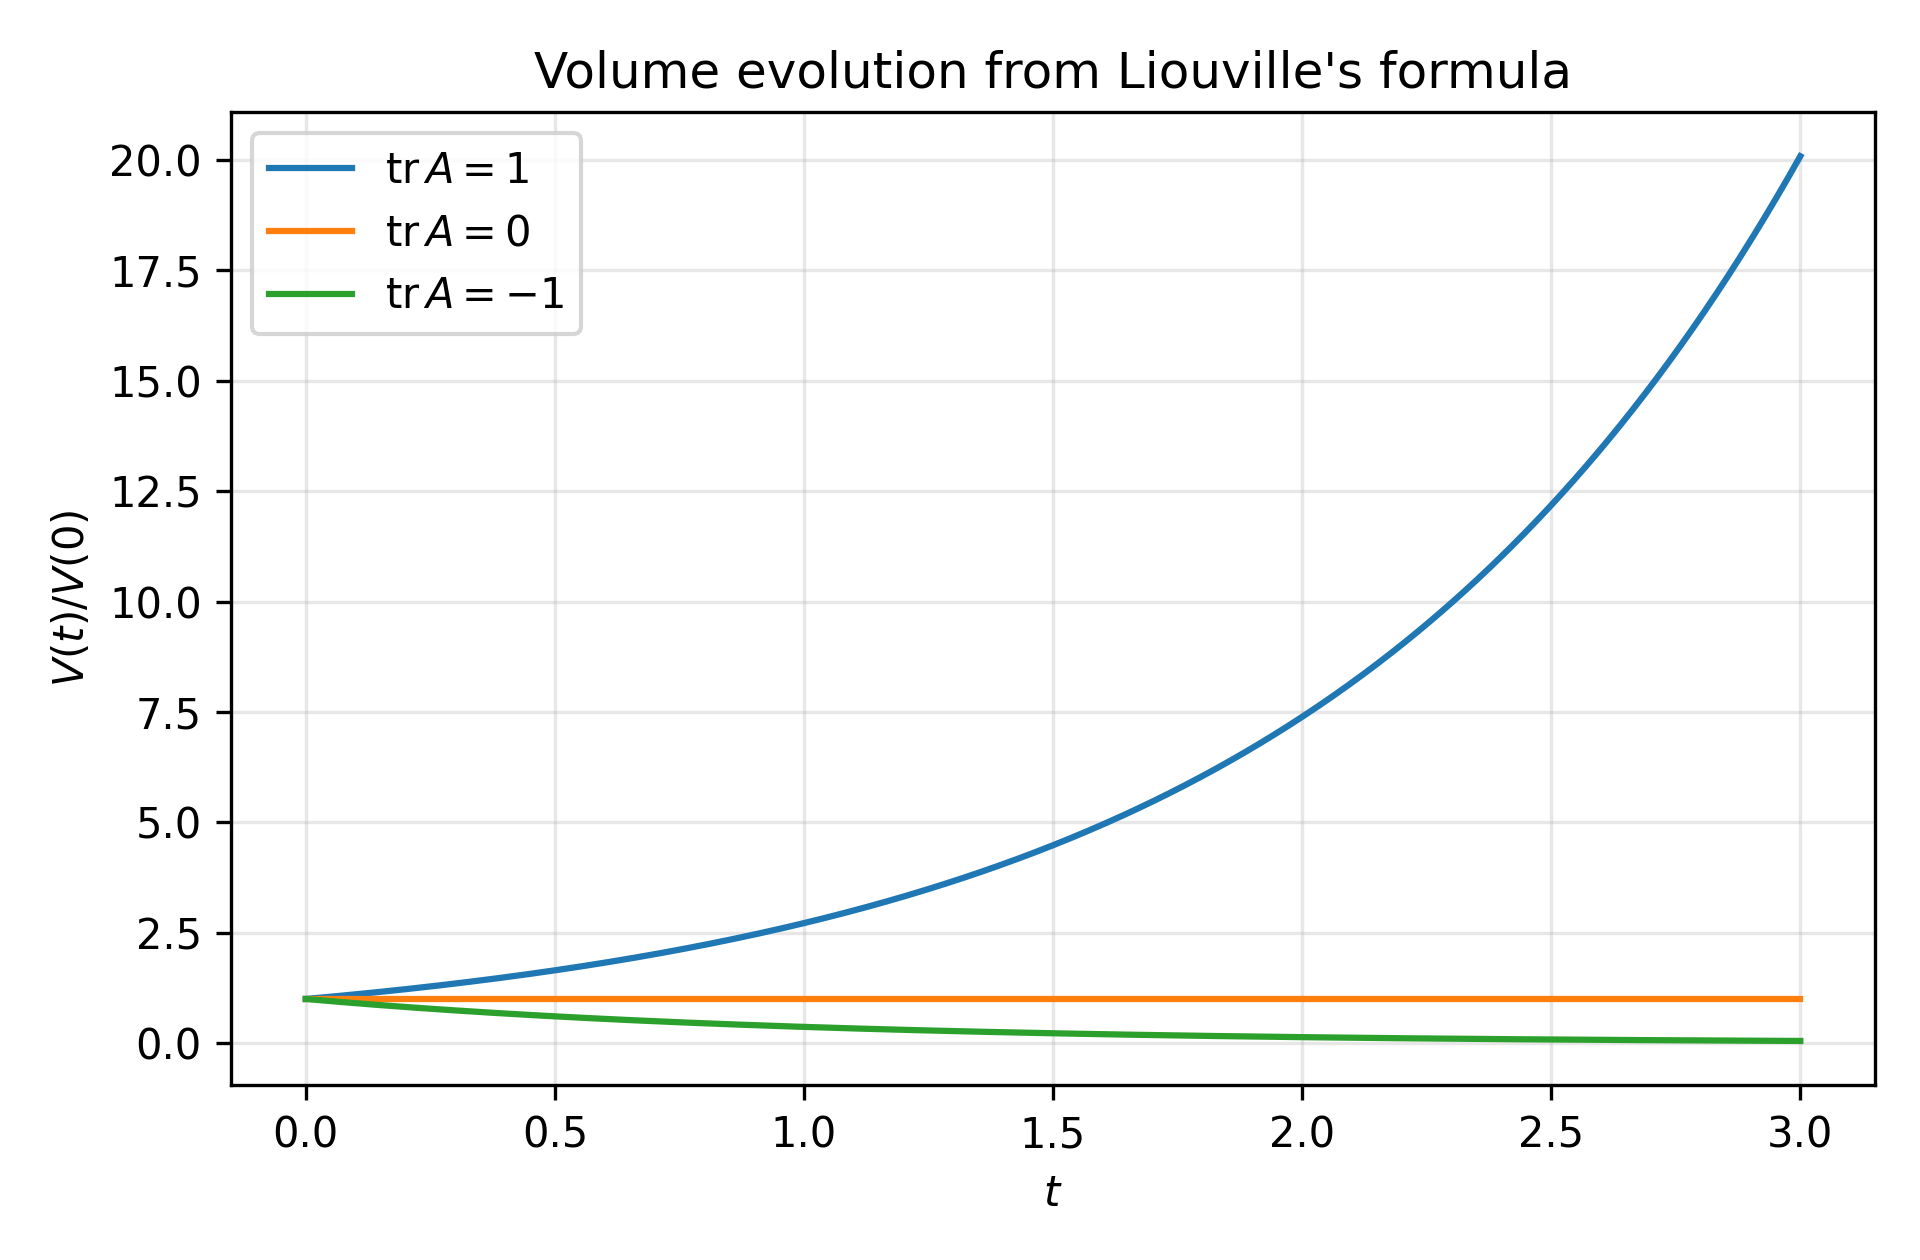
\includegraphics[width=0.72\textwidth]{figures_volume_factors.png}
\caption{Normalized volume factors generated by Eq.~\eqref{eq:constant-trace-volume}. The plotted functions are $V(t)/V(0)=\e^t$ for $c=1$, $V(t)/V(0)=1$ for $c=0$, and $V(t)/V(0)=\e^{-t}$ for $c=-1$. They correspond respectively to constant positive trace, zero trace, and constant negative trace. The plot is generated by the Python program reproduced in Appendix~\ref{app:python-code}.}
\label{fig:volume-factors}
\end{figure}

\subsection{Damped Oscillator and Phase-Space Contraction}

The damped harmonic oscillator gives a mechanical interpretation of a negative matrix trace. Consider a particle whose displacement from equilibrium is $x(t)$ and whose dynamics obey
\be
x''+2\gamma x'+\omega_0^2x=0,
\lb{eq:damped-oscillator}
\ee
where $\omega_0>0$ is the undamped natural angular frequency and $\gamma\geq0$ is the damping rate. The equation is linear and autonomous, but it is second order. To place it in the framework of Liouville's formula, define the velocity $v=x'$ and the phase-space state $\mathbf{z}=(x,v)^{\mathsf T}$. The single second-order equation is then equivalent to
\be
\mathbf{z}'
=
\begin{pmatrix}
0 & 1\\
-\omega_0^2 & -2\gamma
\end{pmatrix}
\mathbf{z}.
\lb{eq:damped-first-order}
\ee
The first row is the kinematic identity $x'=v$, whereas the second row reproduces the dynamical equation $v'=-\omega_0^2x-2\gamma v$. This state-space representation is used in classical mechanics and dynamical-systems treatments of linear oscillations \cite{goldstein2002,hirsch2013}.

The coefficient matrix has trace $-2\gamma$. For the normalized state-transition matrix $\Phi(0)=I_2$, Liouville's formula therefore gives
\be
\det\Phi(t)=\e^{-2\gamma t}.
\lb{eq:damped-determinant}
\ee
This determinant should not be interpreted as the area of one trajectory, because a single trajectory is a one-dimensional curve in the $(x,v)$ plane. Instead, consider any measurable planar region of initial conditions with finite area. The linear flow maps the entire region into another region whose area is multiplied exactly by $\det\Phi(t)$. When $\gamma=0$, the trace vanishes and the phase-space area is preserved. When $\gamma>0$, the determinant decreases exponentially, so every finite patch of initial states contracts at the rate $2\gamma$. The result provides a geometric measure of dissipation that is independent of the detailed phase of any individual oscillator.

This area contraction is related to, but distinct from, mechanical-energy decay. The energy of the oscillator is
\be
E(t)=\frac{1}{2}v^2+\frac{1}{2}\omega_0^2x^2,
\lb{eq:oscillator-energy}
\ee
and differentiation along a solution gives $E'=-2\gamma v^2\leq0$. Energy therefore decreases at a state-dependent instantaneous rate, whereas the phase-space area of a bundle of initial conditions decreases with the factor $\e^{-2\gamma t}$. Liouville's formula obtains this geometric statement from the trace of the first-order system.

Figure~\ref{fig:oscillator-phase-space} is generated by integrating Eq.~\eqref{eq:damped-oscillator} with $\omega_0=1$, initial conditions $x(0)=1$ and $x'(0)=0$, and two damping values, $\gamma=0$ and $\gamma=0.12$. The plotted functions are the parametric trajectories $(x(t),x'(t))$ in phase space. For $\gamma=0$, the trajectory is closed because the undamped oscillator conserves energy. For $\gamma=0.12$, the trajectory spirals inward as energy is dissipated. The corresponding coefficient matrix has trace $-0.24$, so Eq.~\eqref{eq:damped-determinant} predicts the area factor $\e^{-0.24t}$ for any finite measurable patch of initial conditions.

\begin{figure}[ht]
\centering
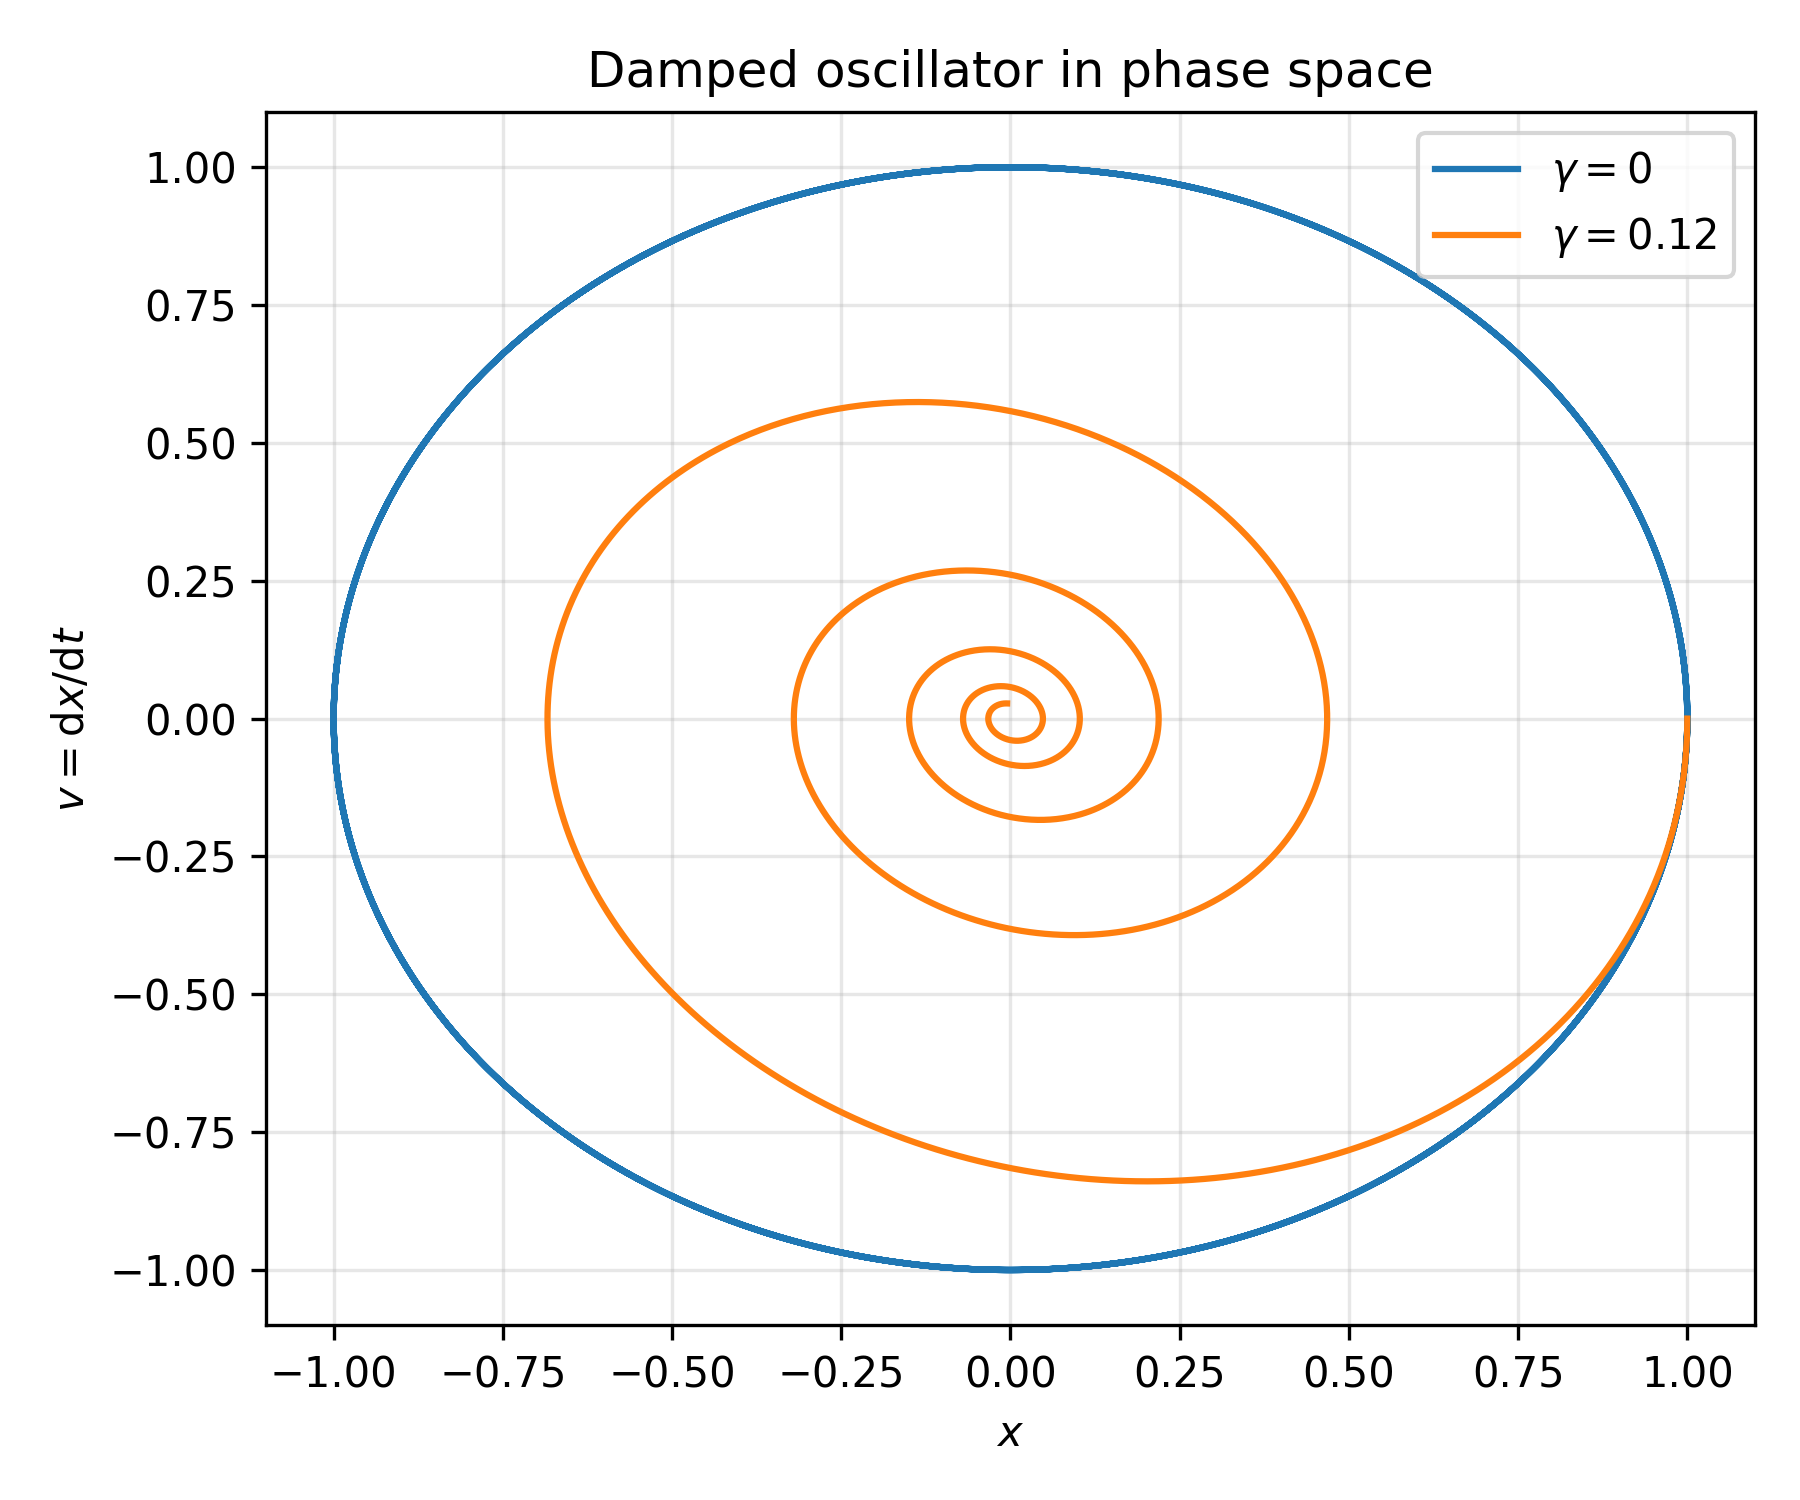
\includegraphics[width=0.68\textwidth]{figures_oscillator_phase_space.png}
\caption{Phase-space trajectories $(x(t),x'(t))$ generated by $x''+2\gamma x'+x=0$ with $x(0)=1$ and $x'(0)=0$. The closed curve uses $\gamma=0$; the inward spiral uses $\gamma=0.12$. For the damped system, the coefficient matrix has trace $-0.24$, so Liouville's formula gives the phase-space area factor $\det\Phi(t)=\e^{-0.24t}$. The figure displays representative trajectories, while the determinant gives the exact area factor for any finite measurable region of initial conditions. The computational procedure is implemented in Appendix~\ref{app:python-code}.}
\label{fig:oscillator-phase-space}
\end{figure}

The area contraction predicted by the theorem can be illustrated with a two-dimensional set of initial states. Under the transition matrix, the unit disk becomes an ellipse whose semiaxes are the singular values $\sigma_1(t)$ and $\sigma_2(t)$ of $\Phi(t,0)$, as established by Eq.~\eqref{eq:polar-volume}. Its exact area is therefore
\be
V_{\rm disk}(t)=\pi\sigma_1(t)\sigma_2(t)=\pi|\det\Phi(t,0)|=\pi\e^{-2\gamma t}.
\lb{eq:oscillator-ellipse-area}
\ee
For Figure~\ref{fig:oscillator-area}, this analytic identity is complemented by a computational consistency check. The unit circle is sampled at $N=720$ equally spaced angles, and the resulting polygon is transformed by $\Phi(t,0)=\exp(tA)$ computed with \texttt{scipy.linalg.expm}. Both the initial polygonal area $\mathcal A_{\rm poly}(0)$ and the transformed polygonal area $\mathcal A_{\rm poly}(t)$ are calculated by the shoelace formula. Since a linear map multiplies every polygonal area by $|\det\Phi|$, the ratio $\mathcal A_{\rm poly}(t)/\mathcal A_{\rm poly}(0)$ has no circle-discretization error; any residual numerical discrepancy reflects the evaluation of the matrix exponential and floating-point arithmetic, rather than an independent test of the geometric area identity.

\begin{figure}[ht]
\centering
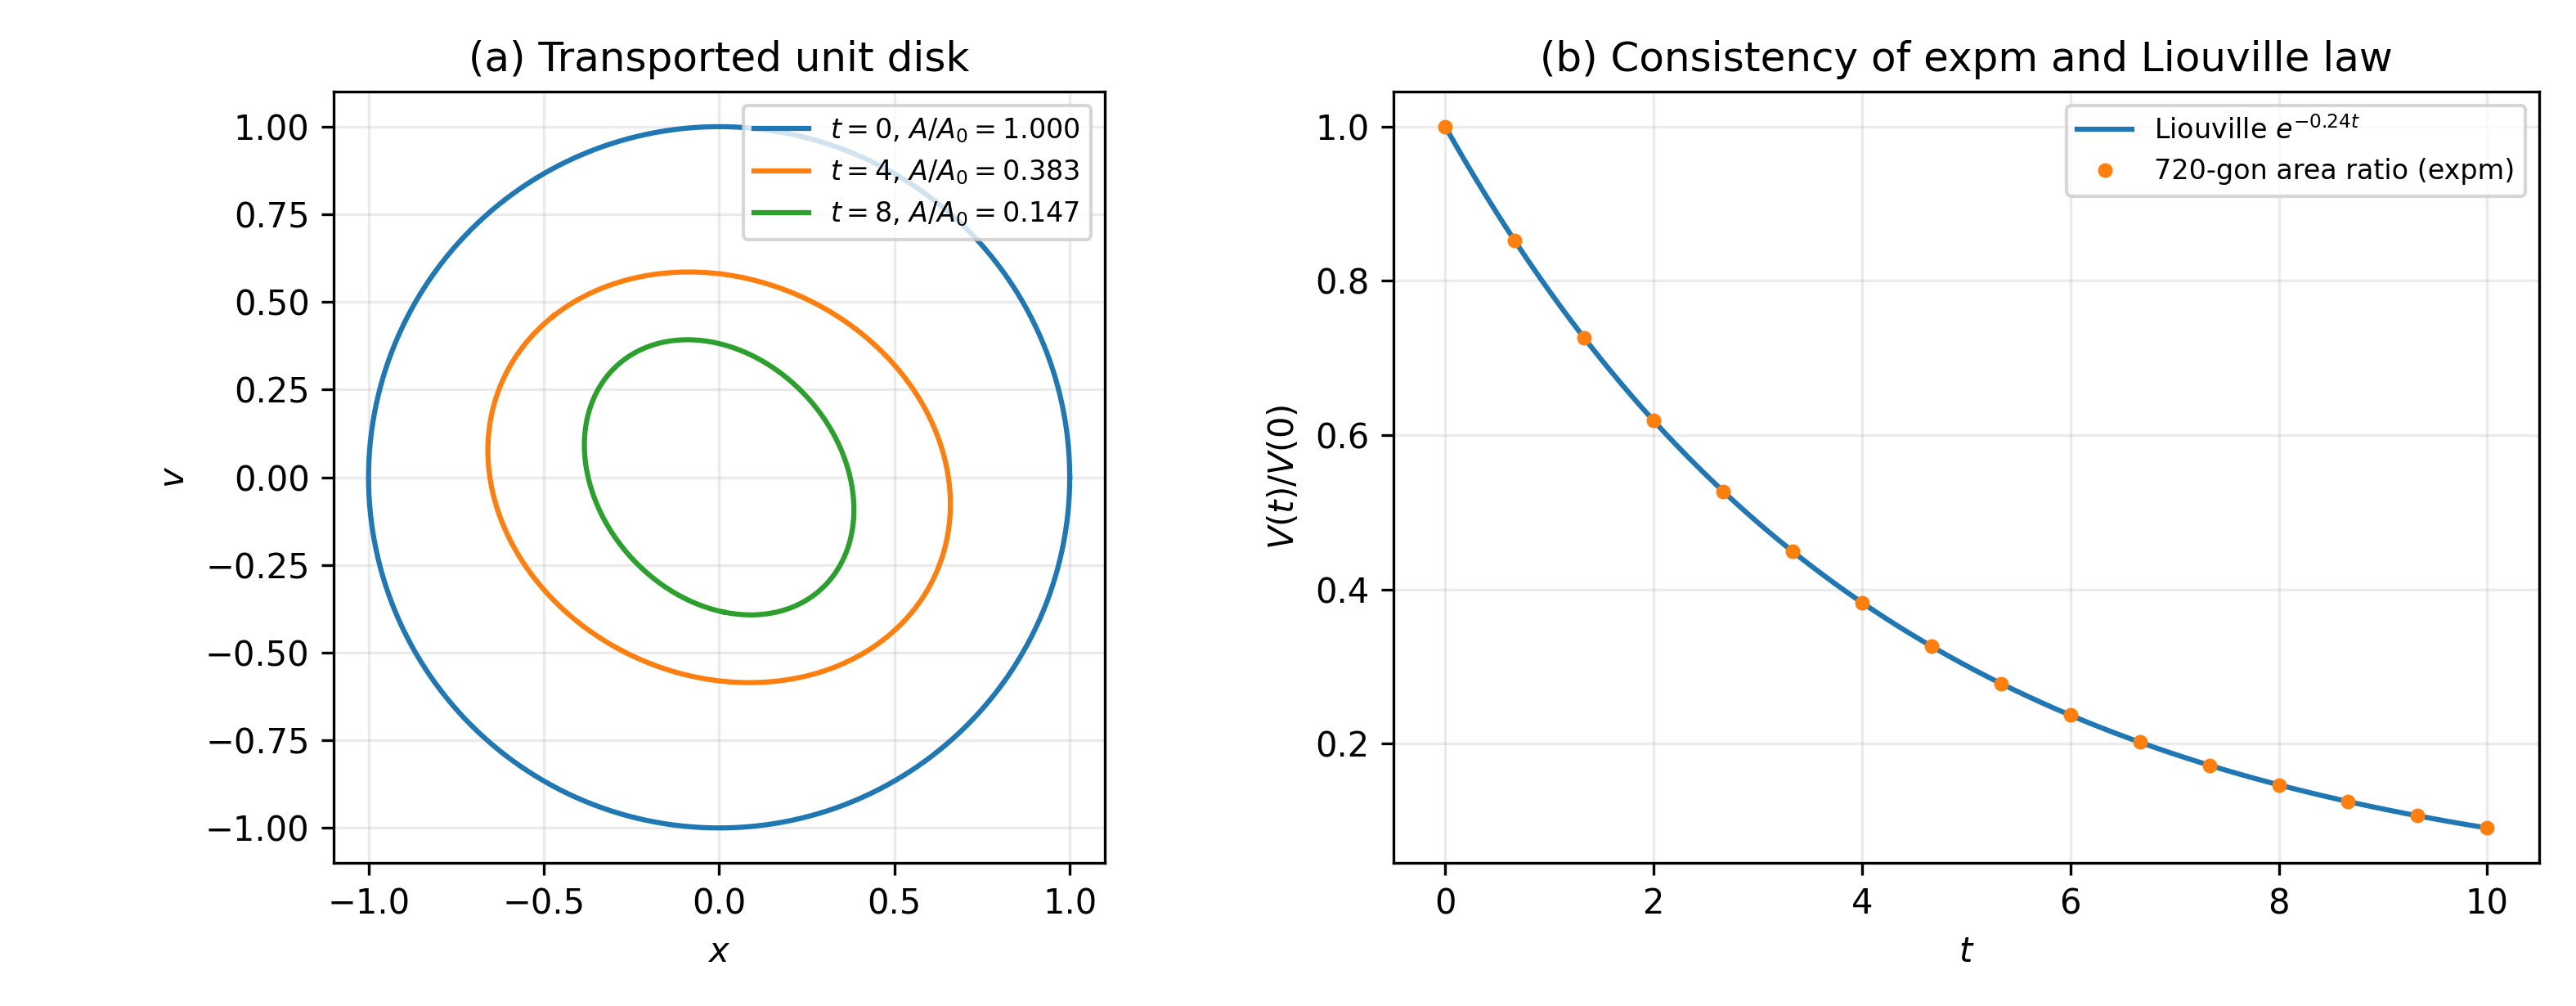
\includegraphics[width=0.94\textwidth]{figures_oscillator_area.png}
\caption{(a) Linear images of the unit-circle boundary under the oscillator flow with $\omega_0=1$ and $\gamma=0.12$. (b) Ratios $\mathcal A_{\rm poly}(t)/\mathcal A_{\rm poly}(0)$ of shoelace areas for a 720-vertex polygon and its images (markers), compared with $\det\Phi(t,0)=\exp(-0.24t)$ (curve). Both polygonal areas use the same discretization; the transition matrix is evaluated by \texttt{scipy.linalg.expm}. Thus the plotted agreement is a numerical consistency check of the computed propagator, with residual differences governed by floating-point evaluation, rather than an independent geometric proof. The complete Python implementation appears in Appendix~\ref{app:python-code}.}
\label{fig:oscillator-area}
\end{figure}


\subsection{Periodic Oscillators and Parametric Stability}

A periodically modulated oscillator provides a direct physical use of the Floquet result in Sec.~\ref{sec:linear-consequences}. Consider
\be
x''+2\gamma x'+\bigl[\omega_0^2+\varepsilon\cos(\Omega t)\bigr]x=0,
\lb{eq:parametric-oscillator}
\ee
where the coefficient matrix in the state vector $\mathbf z=(x,x')^{\mathsf T}$ is
\be
A(t)=
\begin{pmatrix}
0 & 1\\
-[\omega_0^2+\varepsilon\cos(\Omega t)] & -2\gamma
\end{pmatrix}.
\lb{eq:parametric-A}
\ee
The period is $T=2\pi/\Omega$ and $\tr A=-2\gamma$. If $M$ denotes the monodromy matrix over one forcing period, Eq.~\eqref{eq:floquet-product} gives
\be
\det M=\mu_1\mu_2=\e^{-2\gamma T}.
\lb{eq:parametric-multipliers}
\ee
For the undamped parametric oscillator, $\gamma=0$ and the Floquet multipliers satisfy $\mu_1\mu_2=1$. Instability may still occur because one multiplier can move outside the unit circle while the other moves inside by the reciprocal factor. With damping, the determinant constraint still does not determine stability by itself. A practical criterion requires the trace of the monodromy matrix as an additional scalar invariant. With $S=\tr M$ and $D=\det M=\exp(-2\gamma T)$, the characteristic equation is
\be
\mu^2-S\mu+D=0.
\lb{eq:parametric-characteristic}
\ee
Without damping, $D=1$: if $|S|<2$, the multipliers are distinct and lie on the unit circle, whereas $|S|>2$ gives an unstable reciprocal real pair. The boundary $|S|=2$ requires examination of the Jordan form. For positive damping, $0<D<1$, the two multipliers are strictly inside the unit circle if and only if $|S|<1+D$. If $|S|>1+D$, at least one multiplier has modulus greater than one. Equality is a boundary case requiring a separate discussion. Thus Liouville's determinant constraint becomes an operational stability criterion when supplemented by the monodromy trace \cite{yakubovich1975,teschl2012}.

\subsection{Hamiltonian Flow}

Let $\mathbf{z}=(\mathbf{q},\mathbf{p})^{\mathsf T}\in\R^{2m}$ contain generalized coordinates and conjugate momenta. For a quadratic Hamiltonian
\be
\mathcal{H}(\mathbf{z})
=
\frac{1}{2}\mathbf{z}^{\mathsf T}K\mathbf{z},
\lb{eq:quadratic-hamiltonian}
\ee
where $K=K^{\mathsf T}$ is the symmetric Hessian matrix of the quadratic Hamiltonian. Hamilton's equations can then be written as the linear system
\be
\mathbf{z}'=JK\mathbf{z}.
\lb{eq:linear-hamiltonian}
\ee
The matrix that converts the gradient of the Hamiltonian into the canonical Hamiltonian vector field is
\be
J=
\begin{pmatrix}
0 & I_m\\
-I_m & 0
\end{pmatrix}.
\lb{eq:symplectic-J}
\ee
This is the canonical symplectic matrix. Its skew symmetry, together with the symmetry of $K$, immediately constrains the trace of the generator. Since $J^{\mathsf T}=-J$ and $K^{\mathsf T}=K$,
\be
\tr(JK)
=
\tr[(JK)^{\mathsf T}]
=
-\tr(KJ).
\lb{eq:ham-trace1}
\ee
Cyclicity identifies $\tr(KJ)$ with $\tr(JK)$, while transposition supplied the opposite sign; hence the only possibility is $\tr(JK)=0$. Liouville's formula then fixes the phase-space volume factor as
\be
\det\Phi(t)=1.
\lb{eq:ham-det}
\ee
Here the transition matrix is normalized by $\Phi(0)=I_{2m}$. The determinant statement follows from a stronger structure. Because $A=JK$ with $K^{\mathsf T}=K$ and $J^{\mathsf T}=-J$, one has
\be
A^{\mathsf T}J+JA=0.
\lb{eq:ham-generator-symplectic}
\ee
Volume preservation is only one consequence of Hamiltonian structure. To expose the stronger symplectic invariant, differentiate the bilinear form $\Phi^{\mathsf T}J\Phi$ along the flow:
\be
\frac{\dd}{\dd t}(\Phi^{\mathsf T}J\Phi)
=
\Phi^{\mathsf T}(A^{\mathsf T}J+JA)\Phi
=0.
\lb{eq:ham-symplectic-derivative}
\ee
The derivative vanishes, so this matrix-valued quantity is constant. Evaluating that constant at the normalized initial condition $\Phi(0)=I_{2m}$ gives
\be
\Phi^{\mathsf T}(t)J\Phi(t)=J,
\lb{eq:ham-symplectic}
\ee
so the flow is symplectic. Taking determinants gives $(\det\Phi)^2=1$; continuity together with $\det\Phi(0)=1$ selects $\det\Phi(t)=1$. Liouville's formula therefore reproduces the volume consequence of symplecticity, while Eq.~\eqref{eq:ham-symplectic} contains additional information concerning the preservation of the symplectic two-form \cite{goldstein2002,arnold_mechanics1989}.

The quadratic assumption is unnecessary for volume preservation. For a twice continuously differentiable Hamiltonian $\mathcal H:\R^{2m}\to\R$, the nonlinear Hamiltonian field is $\mathbf f(\mathbf z)=J\nabla\mathcal H(\mathbf z)$. Its derivative equals $J\,\operatorname{Hess}\mathcal H$, with a symmetric Hessian. Since $J$ is skew-symmetric, the same trace argument used above yields
\be
\nabla\cdot\left(J\nabla\mathcal H\right)
=\tr\!\left(J\operatorname{Hess}\mathcal H\right)=0.
\lb{eq:ham-general-divergence}
\ee
The nonlinear-flow formula of Sec.~7 then implies $\det D\varphi_{t,t_0}=1$ wherever the flow exists, and the change-of-variables theorem gives preservation of phase-space volume for transported measurable regions. This is the Hamiltonian Liouville theorem, which follows from the determinant evolution of the variational equation. It should be distinguished terminologically from the Abel--Liouville formula for a linear system's fundamental matrix.

\subsection{Continuum Mechanics}

Let $\mathbf{X}$ be a material coordinate in a reference configuration and let $\mathbf{x}=\boldsymbol{\chi}(\mathbf{X},t)$ be the current position. The deformation gradient is
\be
F(\mathbf{X},t)
=
\frac{\partial\boldsymbol{\chi}}{\partial\mathbf{X}}.
\lb{eq:def-gradient}
\ee
Local volume change is encoded by the determinant of this deformation gradient. To distinguish that scalar Jacobian from the symplectic matrix $J$ used above, define
\be
\mathcal{J}(\mathbf{X},t)=\det F(\mathbf{X},t).
\lb{eq:def-jacobian}
\ee
The scalar $\mathcal{J}$ measures the local ratio of current to reference volume; the calligraphic notation avoids confusion with the symplectic matrix $J$ introduced in the preceding subsection. If $\mathbf{v}(\mathbf{x},t)$ is the spatial velocity, define the velocity-gradient tensor
\be
L(\mathbf{x},t)
=
\frac{\partial\mathbf{v}}{\partial\mathbf{x}}.
\lb{eq:velocity-gradient}
\ee
Differentiating the spatial derivative of the motion at fixed material coordinate and applying the chain rule relates the deformation gradient to the spatial velocity gradient. The resulting kinematic identity, with the spatial velocity gradient evaluated at the current position of the material point, is
\be
F'(\mathbf X,t)
=
L(\boldsymbol{\chi}(\mathbf X,t),t)F(\mathbf X,t).
\lb{eq:F-kinematics}
\ee
Here the prime means the time derivative at fixed material label $\mathbf{X}$, equivalently the material time derivative of $F$ along the motion. This follows by differentiating $F=\partial\boldsymbol{\chi}/\partial\mathbf{X}$ with respect to time, using $\mathbf{v}=\partial\boldsymbol{\chi}/\partial t$, and applying the chain rule to express the spatial derivative of $\mathbf{v}$ through $L$. Applying Jacobi's formula to $\mathcal{J}=\det F$ gives
\be
\mathcal{J}'
=
\mathcal{J}\tr(F^{-1}F').
\lb{eq:J-jacobi}
\ee
Jacobi's formula converts this matrix kinematics into a scalar law for local volume change. Substitution of Eq.~\eqref{eq:F-kinematics}, followed by similarity invariance of the trace, yields the local volume-rate law along the material trajectory,
\be
\mathcal{J}'(\mathbf X,t)
=
\mathcal{J}(\mathbf X,t)\,\tr L(\boldsymbol{\chi}(\mathbf X,t),t)
=
\mathcal{J}(\mathbf X,t)\,\nabla\cdot\mathbf{v}(\boldsymbol{\chi}(\mathbf X,t),t).
\lb{eq:J-continuum}
\ee
Hence local incompressibility, $\nabla\cdot\mathbf{v}=0$, implies constant $\mathcal{J}$; with the reference normalization $\mathcal{J}=1$, material volume is preserved \cite{gurtin2010}.

\subsection{Cosmology}

The Friedmann--Lema\^itre--Robertson--Walker metric defines the FLRW spacetime. It describes a homogeneous and isotropic universe. We adopt metric signature $(-,+,+,+)$, units with the speed of light $c=1$, cosmic time $t$, comoving radial coordinate $r$, and angular coordinates $(\theta,\phi)$. The FLRW line element is \cite{weinberg2008,dodelson2003,mukhanov2005,peebles1993}
\be
\dd s^2
=
-\dd t^2
+
a^2(t)
\left[
\frac{\dd r^2}{1-kr^2}
+
r^2\dd\theta^2
+
r^2\sin^2\theta\,\dd\phi^2
\right],
\lb{eq:flrw-metric}
\ee
where $a(t)>0$ is the scale factor and $k$ is the constant spatial-curvature parameter, conventionally normalized to $k=-1,0,+1$ for negative-, zero-, and positive-curvature spatial geometries, respectively.

At fixed cosmic time, the induced three-dimensional spatial metric $h_{ij}$ is the positive-definite spatial part of Eq.~\eqref{eq:flrw-metric}. In the coordinates $(r,\theta,\phi)$ its determinant is
\be
\det h
=
\frac{a^6(t)r^4\sin^2\theta}{1-kr^2}.
\lb{eq:flrw-hdet}
\ee
The Riemannian volume element on a spatial hypersurface is the square root of the metric determinant times the coordinate volume element. Substituting the FLRW spatial determinant therefore gives
\be
\dd V_{\rm phys}
=
\sqrt{\det h}\,\dd r\,\dd\theta\,\dd\phi
=
a^3(t)
\frac{r^2\sin\theta}{\sqrt{1-kr^2}}
\dd r\,\dd\theta\,\dd\phi.
\lb{eq:flrw-volume-element}
\ee
The factor multiplying the coordinate element separates into a time-dependent factor $a^3(t)$ and a purely comoving spatial factor. For any fixed comoving region $\mathcal{C}$,
\be
V_{\rm phys}(t)
=
a^3(t)V_{\rm com},
\lb{eq:flrw-volume-scaling}
\ee
where $V_{\rm com}$ denotes the time-independent integral of the remaining spatial measure over $\mathcal{C}$. Equation~\eqref{eq:flrw-volume-scaling} is the geometric origin of the cubic volume scaling in an isotropically expanding universe.

To connect the metric result with a simple matrix representation, use the spatially flat chart $k=0$ and comoving Cartesian coordinates $\mathbf{X}\in\R^3$. This restriction simplifies the coordinate demonstration; the $a^3$ volume factor derived from the metric above holds for all three spatial curvatures. In this chart physical separations are
\be
\mathbf{r}(t)=a(t)\mathbf{X}.
\lb{eq:cosmo-map}
\ee
Choose a reference time $t_0$. The normalized linear map between physical separations at $t_0$ and $t$ is
\be
\Phi(t,t_0)
=
\frac{a(t)}{a(t_0)}I_3.
\lb{eq:cosmo-transition}
\ee
Differentiating Eq.~\eqref{eq:cosmo-map} while keeping the comoving coordinate $\mathbf{X}$ fixed gives
\be
\mathbf{r}'(t)=a'(t)\mathbf{X}.
\lb{eq:cosmo-derivative1}
\ee
For a comoving particle the coordinate $\mathbf X$ is constant, so $\mathbf X=\mathbf r/a$ can be substituted back into the differentiated relation. This rewrites the recession law entirely in terms of the physical separation:
\be
\mathbf{r}'(t)=H(t)\mathbf{r}(t).
\lb{eq:hubble-flow}
\ee
The proportionality coefficient between physical separation and recession velocity is the Hubble parameter, defined by
\be
H(t)=\frac{a'(t)}{a(t)}.
\lb{eq:hubble-parameter}
\ee
With this definition, the separation field is a linear isotropic system whose coefficient matrix is
\be
A(t)=H(t)I_3,
\qquad
\tr A(t)=3H(t).
\lb{eq:cosmo-A}
\ee
Although $H(t)$ generally varies with cosmic time, the trace retains the simple form $3H(t)$. Liouville's formula therefore determines the transition determinant without assuming an autonomous system:
\be
\det\Phi(t,t_0)
=
\exp\left[
3\int_{t_0}^{t}H(s)\,\dd s
\right].
\lb{eq:cosmo-liouville1}
\ee
The definition $H=a'/a$ makes the time integral elementary because the integrand is the logarithmic derivative of the scale factor. Hence
\be
\int_{t_0}^{t}H(s)\,\dd s
=
\ln\frac{a(t)}{a(t_0)}.
\lb{eq:cosmo-H-integral}
\ee
Substituting the evaluated integral into Liouville's formula converts the accumulated Hubble rate into the finite ratio of scale factors, giving
\be
\det\Phi(t,t_0)
=
\left[
\frac{a(t)}{a(t_0)}
\right]^3.
\lb{eq:cosmo-liouville2}
\ee
This agrees with the volume factor obtained from the FLRW spatial metric in Eq.~\eqref{eq:flrw-volume-scaling}. The calculation shows that the same determinant--trace identity reproduces the physical $a^3$ scaling of a comoving volume. Treatments of FLRW geometry and cosmic expansion include Weinberg, Peebles, Mukhanov, and Dodelson \cite{weinberg2008,peebles1993,mukhanov2005,dodelson2003}.

The same result can be stated covariantly in terms of the comoving cosmological congruence. In the coordinates of Eq.~\eqref{eq:flrw-metric}, comoving observers have four-velocity $u^\mu=(1,0,0,0)$. The expansion scalar is $\Theta=\nabla_\mu u^\mu$. From the metric determinant $g=-a^6(t)r^4\sin^2\theta/(1-kr^2)$, the covariant divergence can be calculated explicitly. Since the spatial factor in $\sqrt{-g}$ is independent of $t$ and $u^t=1$,
\be
\Theta
=\frac{1}{\sqrt{-g}}\partial_\mu(\sqrt{-g}\,u^\mu)
=\frac{1}{a^3(t)}\frac{\dd}{\dd t}a^3(t)
=3H(t).
\lb{eq:flrw-expansion-scalar}
\ee
The physical volume transported with the congruence therefore satisfies
\be
\frac{1}{V_{\rm phys}}\frac{\dd V_{\rm phys}}{\dd t}=\Theta=3H(t),
\lb{eq:flrw-covariant-volume}
\ee
which is the relativistic form of Eq.~\eqref{eq:relative-volume-rate}. In the matrix description, the same scalar appears as $\tr A=3H$; in the spacetime description, it appears as the expansion scalar of the comoving four-velocity field. This equivalence makes the Liouville interpretation of cosmological volume expansion geometrically explicit. \cite{weinberg2008,mukhanov2005}

%%%%%%%%%%%%%%%%%%%%%%%%%%%%%%%%%%%%%%%%%%%%%%%%%%%%%%%%%%%%%%%%%%%%%%%


%%%%%%%%%%%%%%%%%%%%%%%%%%%%%%%%%%%%%%%%%%%%%%%%%%%%%%%%%%%%%%%%%%%%%%%
\section{Conclusion}

The paper develops Liouville's formula as a relation between three levels of a linear dynamical system. The coefficient matrix $A(t)$ specifies the instantaneous generator, the transition matrix $\Phi(t,t_0)$ contains the complete finite-time deformation, and its determinant retains the scalar component associated with oriented volume. The formula shows that this volume information is determined by the time integral of $\tr A(t)$ even when the full transition matrix is unavailable.

This separation explains both the reach and the limitation of the result. A zero trace enforces volume preservation but does not distinguish rotation, shear, or compensating directional stretching. For periodic systems, the same scalar constraint fixes the product of Floquet multipliers rather than each multiplier separately. For nonlinear flows, the variational equation transfers the determinant--trace relation to the Jacobian of the flow, where the trace becomes the divergence. The applications in fluid mechanics, oscillation theory, Hamiltonian dynamics, continuum mechanics, and cosmology are instances of the same local-to-finite-time mechanism.

Abel's identity supplies the scalar prototype, Jacobi's formula supplies the determinant derivative, and geometric transport supplies the interpretation. Together they identify the trace as an instantaneous logarithmic volume rate and the determinant of the fundamental or transition matrix as its accumulated finite-time effect.

\appendix
\section{Python Code for Reproducing the Figures}
\label{app:python-code}

This appendix reproduces, without omissions, the Python source used to generate Figs.~\ref{fig:volume-factors}, \ref{fig:oscillator-phase-space}, and \ref{fig:oscillator-area}. The program requires NumPy, SciPy, and Matplotlib, and writes the output images to the directory containing the script. The first routine plots the analytical volume factors for constant matrix trace, whereas the second integrates the damped oscillator using \texttt{scipy.integrate.solve\_ivp} with the tolerances specified in the source.

The third routine applies \texttt{scipy.linalg.expm} to the vertices of a regular polygon and compares the ratio of transported polygonal areas with the determinant predicted by Liouville's formula. Because both areas refer to the same polygon, its discretisation of the unit disk cancels from the ratio. The comparison therefore checks the numerical evaluation of the state-transition matrix against its theoretical determinant rather than supplying an independent geometric proof.

\begin{lstlisting}[style=paperpython,caption={Complete source of \texttt{liouville\_examples.py}.},label={lst:python-figures}]
"""Reproduce the numerical figures for the Abel--Liouville pedagogical paper.

Uses NumPy, SciPy and Matplotlib. All files are written beside this script.
"""
from pathlib import Path
import numpy as np
import matplotlib.pyplot as plt
from scipy.integrate import solve_ivp
from scipy.linalg import expm

OUT = Path(__file__).resolve().parent

def plot_volume_factors():
    t = np.linspace(0, 3, 501)
    fig, ax = plt.subplots(figsize=(6.4, 4.2))
    for c in [1, 0, -1]:
        ax.plot(t, np.exp(c*t), label=rf'$\operatorname{{tr}} A={c}$')
    ax.set(xlabel='$t$', ylabel='$V(t)/V(0)$', title='Volume evolution from Liouville\'s formula')
    ax.grid(alpha=.3);ax.legend();fig.tight_layout()
    fig.savefig(OUT/'figures_volume_factors.png', dpi=300)
    plt.close(fig)

def plot_oscillator_phase_space():
    t=np.linspace(0,30,3001)
    fig,ax=plt.subplots(figsize=(6,5))
    for g in [0.,.12]:
        def rhs(t,y): return [y[1],-y[0]-2*g*y[1]]
        sol=solve_ivp(rhs,(0,30),[1,0],t_eval=t,rtol=1e-11,atol=1e-13)
        ax.plot(sol.y[0],sol.y[1],label=rf'$\gamma={g:g}$')
    ax.set(xlabel='$x$',ylabel="$v=\\mathrm{d}x/\\mathrm{d}t$",title='Damped oscillator in phase space')
    ax.grid(alpha=.3);ax.legend();fig.tight_layout()
    fig.savefig(OUT/'figures_oscillator_phase_space.png',dpi=300)
    plt.close(fig)

def polygon_area(coords):
    x,y=coords[0],coords[1]
    return .5*abs(np.dot(x,np.roll(y,-1))-np.dot(y,np.roll(x,-1)))

def plot_oscillator_area():
    """Check expm against Liouville's area law with a fixed 720-gon.

    The shoelace-area ratio of a polygon under a linear map is exactly
    abs(det(map)); no circle-versus-polygon discretization error survives
    this ratio. Residual differences reflect expm and floating-point error.
    """
    gamma=.12
    A=np.array([[0.,1.],[-1.,-2*gamma]])
    theta=np.linspace(0,2*np.pi,720,endpoint=False)
    circle=np.vstack((np.cos(theta),np.sin(theta)))
    unit_area=polygon_area(circle)
    t_sample=np.linspace(0,10,16)
    ratios=[]
    for t in t_sample:
        ell=expm(t*A)@circle
        ratios.append(polygon_area(ell)/unit_area)
    predicted=np.exp(-2*gamma*t_sample)
    assert np.max(abs(np.array(ratios)-predicted))<5e-13
    fig,(ax0,ax1)=plt.subplots(1,2,figsize=(10.5,4.1))
    for t in [0.,4.,8.]:
        ell=expm(t*A)@circle
        ax0.plot(np.r_[ell[0],ell[0,0]],np.r_[ell[1],ell[1,0]],label=f'$t={t:g}$, $A/A_0={np.exp(-.24*t):.3f}$')
    ax0.set(xlabel='$x$',ylabel='$v$',title='(a) Transported unit disk')
    ax0.set_aspect('equal',adjustable='box');ax0.grid(alpha=.25);ax0.legend(fontsize=8)
    t=np.linspace(0,10,500)
    ax1.plot(t,np.exp(-2*gamma*t),label='Liouville $e^{-0.24t}$')
    ax1.plot(t_sample,ratios,'o',markersize=3.3,label='720-gon area ratio (expm)')
    ax1.set(xlabel='$t$',ylabel='$V(t)/V(0)$',title='(b) Consistency of expm and Liouville law')
    ax1.grid(alpha=.25);ax1.legend(fontsize=8)
    fig.tight_layout()
    fig.savefig(OUT/'figures_oscillator_area.png',dpi=300)
    plt.close(fig)

if __name__=='__main__':
    plot_volume_factors()
    plot_oscillator_phase_space()
    plot_oscillator_area()
\end{lstlisting}

\begingroup\small
\begin{thebibliography}{99}

\bibitem{coddington1955}
E. A. Coddington and N. Levinson,
\textit{Theory of Ordinary Differential Equations},
McGraw--Hill, New York, 1955.

\bibitem{hartman2002}
P. Hartman,
\textit{Ordinary Differential Equations}, 2nd ed.,
Classics in Applied Mathematics, Vol.~38,
Society for Industrial and Applied Mathematics, Philadelphia, 2002.

\bibitem{teschl2012}
G. Teschl,
\textit{Ordinary Differential Equations and Dynamical Systems},
Graduate Studies in Mathematics, Vol.~140,
American Mathematical Society, Providence, 2012,
\url{https://www.mat.univie.ac.at/~gerald/ftp/book-ode/}.

\bibitem{horn2013}
R. A. Horn and C. R. Johnson,
\textit{Matrix Analysis}, 2nd ed.,
Cambridge University Press, Cambridge, 2013.

\bibitem{abel1827}
N. H. Abel,
``Ueber einige bestimmte Integrale,''
\textit{Journal f\"ur die reine und angewandte Mathematik},
Vol.~2 (1827), pp.~22--30,
\url{https://doi.org/10.1515/crll.1827.2.22}.

\bibitem{liouville1838}
J. Liouville,
``Note sur la th\'eorie de la variation des constantes arbitraires,''
\textit{Journal de Math\'ematiques Pures et Appliqu\'ees},
S\'erie 1, Vol.~3 (1838), pp.~342--349,
\url{https://numdam.org/item/JMPA_1838_1_3__342_0/}.

\bibitem{jacobi1841}
C. G. J. Jacobi,
``De determinantibus functionalibus,''
\textit{Journal f\"ur die reine und angewandte Mathematik},
Vol.~22 (1841), pp.~319--359,
\url{https://www.degruyterbrill.com/journal/key/crll/1841/22/html}.

\bibitem{dlmf_abel}
NIST Digital Library of Mathematical Functions,
``Differential Equations,'' Sec.~1.13, Eqs.~(1.13.4)--(1.13.5),
\url{https://dlmf.nist.gov/1.13}.

\bibitem{apostol1969}
T. M. Apostol,
\textit{Calculus, Volume II}, 2nd ed.,
Wiley, New York, 1969.

\bibitem{rugh1996}
W. J. Rugh,
\textit{Linear System Theory}, 2nd ed.,
Prentice Hall, Upper Saddle River, NJ, 1996.

\bibitem{brockett1970}
R. W. Brockett,
\textit{Finite Dimensional Linear Systems},
John Wiley \& Sons, New York, 1970.

\bibitem{arnold1992}
V. I. Arnold,
\textit{Ordinary Differential Equations}, 3rd ed.,
Springer-Verlag, Berlin, 1992.

\bibitem{hirsch2013}
M. W. Hirsch, S. Smale, and R. L. Devaney,
\textit{Differential Equations, Dynamical Systems, and an Introduction to Chaos}, 3rd ed.,
Academic Press, Boston, 2013.

\bibitem{yakubovich1975}
V. A. Yakubovich and V. M. Starzhinskii,
\textit{Linear Differential Equations with Periodic Coefficients},
Wiley, New York, 1975.

\bibitem{perko2001}
L. Perko,
\textit{Differential Equations and Dynamical Systems}, 3rd ed.,
Springer, New York, 2001.

\bibitem{batchelor1967}
G. K. Batchelor,
\textit{An Introduction to Fluid Dynamics},
Cambridge University Press, Cambridge, 1967.


\bibitem{goldstein2002}
H. Goldstein, C. Poole, and J. Safko,
\textit{Classical Mechanics}, 3rd ed.,
Addison Wesley, San Francisco, 2002.

\bibitem{arnold_mechanics1989}
V. I. Arnold,
\textit{Mathematical Methods of Classical Mechanics}, 2nd ed.,
Springer, New York, 1989.

\bibitem{gurtin2010}
M. E. Gurtin, E. Fried, and L. Anand,
\textit{The Mechanics and Thermodynamics of Continua},
Cambridge University Press, Cambridge, 2010.

\bibitem{weinberg2008}
S. Weinberg,
\textit{Cosmology},
Oxford University Press, Oxford, 2008.

\bibitem{dodelson2003}
S. Dodelson,
\textit{Modern Cosmology},
Academic Press, San Diego, 2003.

\bibitem{mukhanov2005}
V. Mukhanov,
\textit{Physical Foundations of Cosmology},
Cambridge University Press, Cambridge, 2005.

\bibitem{peebles1993}
P. J. E. Peebles,
\textit{Principles of Physical Cosmology},
Princeton University Press, Princeton, 1993.

\end{thebibliography}
\endgroup

\end{document}
